\documentclass[12pt]{article}
        \usepackage{graphicx,type1cm,eso-pic,color}
        \usepackage{hyperref}
        \usepackage[left=3.0cm,right=3.0cm,top=2cm,bottom=2cm,headheight=13.6pt]{geometry}
        \usepackage{subfigure}

\makeatother


\title{Manual for CLAS12 \\ Ring Imaging Cherenkov Counter}

\author{
%RICH On-Call Cell Phone: 757-810-1489 \\ 
Authors: \\
M. Contalbrigo (mcontalb@jlab.org) \\
V. Kubarovsky (vpk@jlab.org)\\
M. Mirazita (mirazita@jlab.org)\\
F. Benmokhtar (fatiha@jlab.org)\\
J. Goodwill (goodwi12@duq.edu)
}

\date{\today} %01/07/2014


\begin{document}
\maketitle{}

\tableofcontents

%%%%%%%%%%%%%%%%%%%%%%%%%%%%%%%%%%%%%%%%%%%%%%%%%%%%%%%%%%%%%%%
\newpage
   \section{General description of the RICH}

The first module of the CLAS12 Ring Imaging Cherenkov (RICH) detector is installed on the forward carriage in Sector 4, downstream of the third region of drift chambers and just before the Time-Of-Flight (TOF) system.
A second RICH module is foreseen for the starting of operation with transversely polarized target.
It's goal is to provide identification of kaons with respect to pions and protons at a 4~$\sigma$ level in the momentum range between 3 and 8 GeV/c for polar angles up to 35$^o$.
The RICH design incorporates aerogel radiators, visible light photon detectors, and a focusing mirror system which is used to reduce the detection area instrumented by photon detectors to about 1 m$^2$. 
Multi-anode photomultiplier tubes (MAPMTs) Hamamatsu H8500 and H12700 provide the required spatial resolution and match the aerogel Cherenkov light spectrum (visible and near-ultraviolet region). 

The RICH is composed by a large trapezoidal box made in aluminum and carbon fiber, with smaller base of about 0.3 m, a larger base of about 4.2 m, a height of about 3.7 m and a depth of about 1.2 m. 
The total weight is approximately 900 Kg. 
Two drawings of the RICH box frontal and backward views are shown in figure~\ref{fig:RICH_outer}. 


\vspace*{\stretch{1}}      
\begin{figure}[h!]
\center
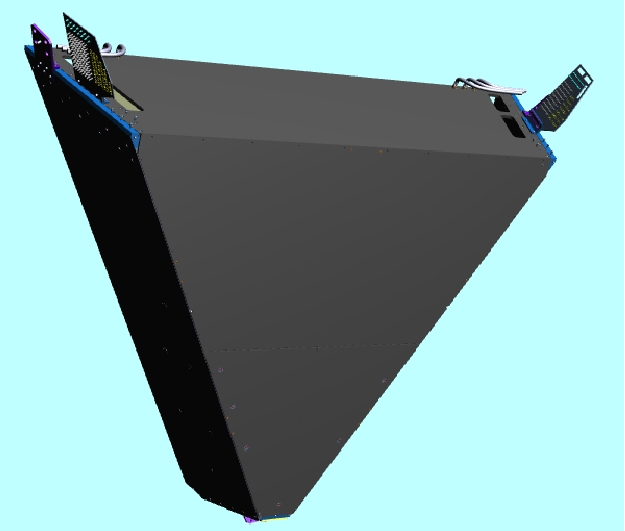
\includegraphics[width=0.53\textwidth]{pics/Rich_frontal.jpg}
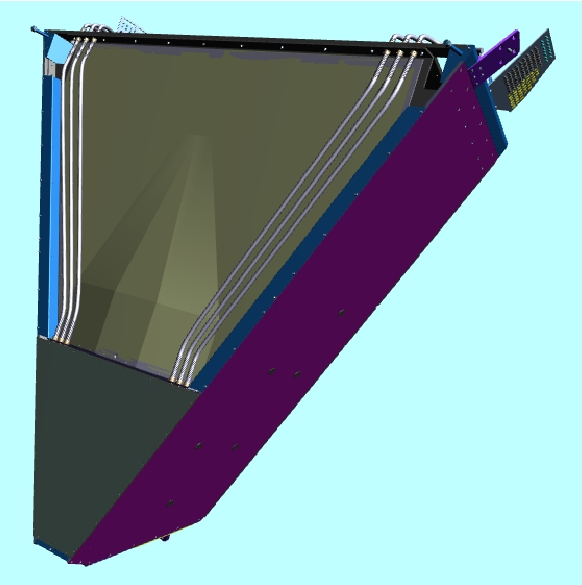
\includegraphics[width=0.46\textwidth]{pics/Rich_back.jpg}
\caption{ \label{fig:RICH_outer} Back and frontal drawings of the RICH module.}
\end{figure}

Inside the RICH box, a number of active elements are installed, namely:
\begin{itemize}
\item{the aerogel radiator;}
\item{the planar and spherical mirrors;}
\item{the MAPMTs and the readout Front-End Electronics (FEE).}
\end{itemize}

A cross section of the RICH showing the inner elements in shown in figure~\ref{fig:RICH_inner}.

\vspace*{\stretch{1}}      
\begin{figure}[h!]
\center
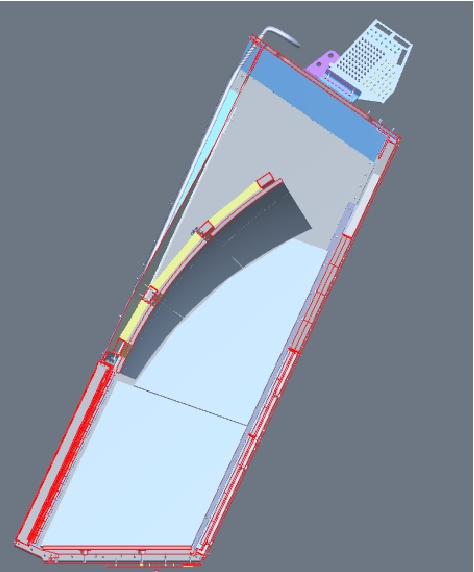
\includegraphics[width=0.9\textwidth]{pics/Rich_lateral.jpg}
\caption{ \label{fig:RICH_inner} Cross section of the RICH.}
\end{figure}

The aerogel is an igrophilic material that absorbs water from the environment humidity, resulting in a reduction of its optical performance.
For this reason, a strict protocol to handle it has been established during the test and assembly.
In addition, the RICH box volume is fluxed with dry nitrogen, in order to prevent water absorption during the operation of the detector.

The detection of the Cherenkov photon is achieved by means of 391 Multi-Anode PhotoMultiplier Tubes (MAPMTs) and the Front-End Electronics (FEE), mounted on a triangular box, about 1.7 m wide, 1.3 m high and about 10 cm thick, that is installed on the lower back of the RICH module.


%%%%%%%%%%%%%%%%%%%%%%%%%%%%%%%%%%%%%%%%%%%%%%%%%%%%%%%%%%%%%%%
%\newpage
{\color{blue}
\section{The RICH Electronics}
}
%=========================================================
\subsection{Photodetectors and Front-End electronics}

The Cherenkov photons are detected by using 391 MAPMTs Hamamatsu H8500 and H12700.
They are mounted on a carbon fiber panel installed on the lower back of the RICH and that also host the Front-End electronics.

Photodetectors and Front-End electronics are organized in tiles housing groups of 2 or 3 MAPMTs, see Fig. \ref{fig:RICH_Electronics} for the 3 MAPMT case.
There are 23 tiles with 2 MAPMTs and 113 tiles with 3 MAPMTs.
Each tile is composed by an adapter board, an ASIC board and a FPGA board.

The adapter board ensure the connection between the MAPMTs and the ASIC board and also supplies the HV to the MAPMTs.
The ASIC board houses the MAROC3 chips, one per MAPMT.
The Multi Anode Read Out Chip (MAROC3) is a 64 channel Application Specific Integrated Circuit (ASIC), able to discriminate the 64 channels PMT output signals and produce 64 corresponding binary outputs. 
The chip provides single channel adjustable gain in the range between 0 and 4 and one adjustable threshold level.
The MAROC3 chip is configured, controlled and readout by an FPGA, that also provide the LV supply to the the ASIC board and the interface with the DAQ via optical link.



\vspace*{\stretch{1}}      
\begin{figure}[h!]
\center
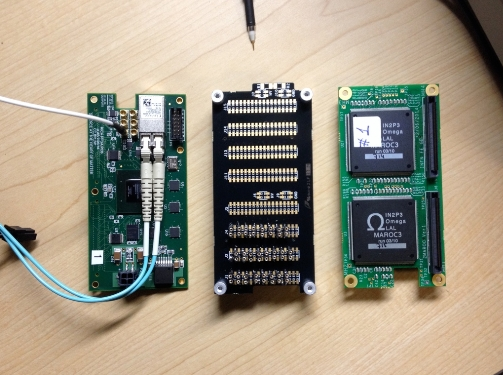
\includegraphics[width=0.46\textwidth]{pics/RICH_ElectronicsBoards.jpg}
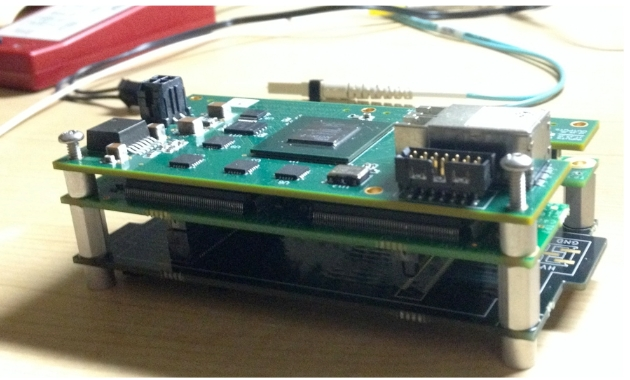
\includegraphics[width=0.46\textwidth]{pics/RICH_ElectronicsAssembled.jpg}
\caption{ \label{fig:RICH_Electronics} The RICH electronic boards for the 2 MAPMT case (left) and the tile fully assembled (right).}
\end{figure}

The list of the components of the RICH readout electronics is reported in figure~\ref{fig:RICH_services}.

\vspace*{\stretch{1}}      
\begin{figure}[h!]
\center
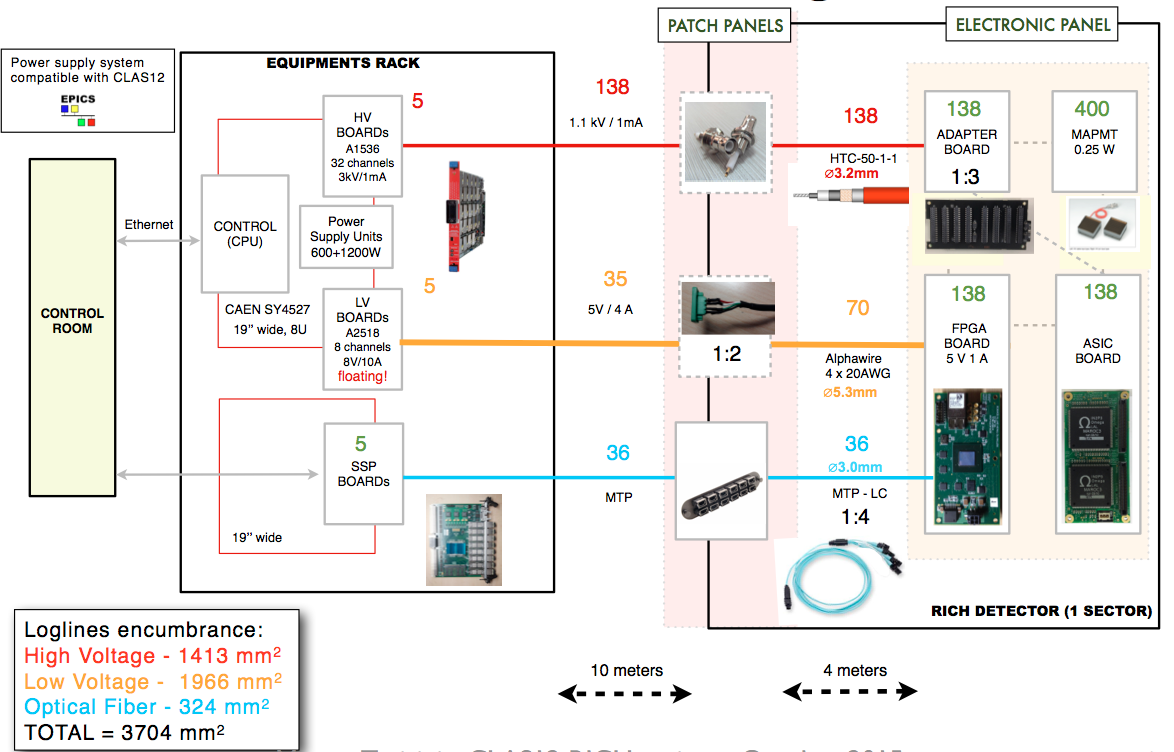
\includegraphics[width=0.99\textwidth]{pics/Services_HV_LV.png}
\caption{ \label{fig:RICH_services} Sketch of the RICH services: LV, HV supply lines and DAQ optical link.}
\end{figure}



%=========================================================
\subsection{HV and LV Power Supply}

The low voltage and high voltage power supply is a CAEN SY4527, see Fig.~\ref{Fig:SY4527}. 

\begin{figure}[htbp]
\center
%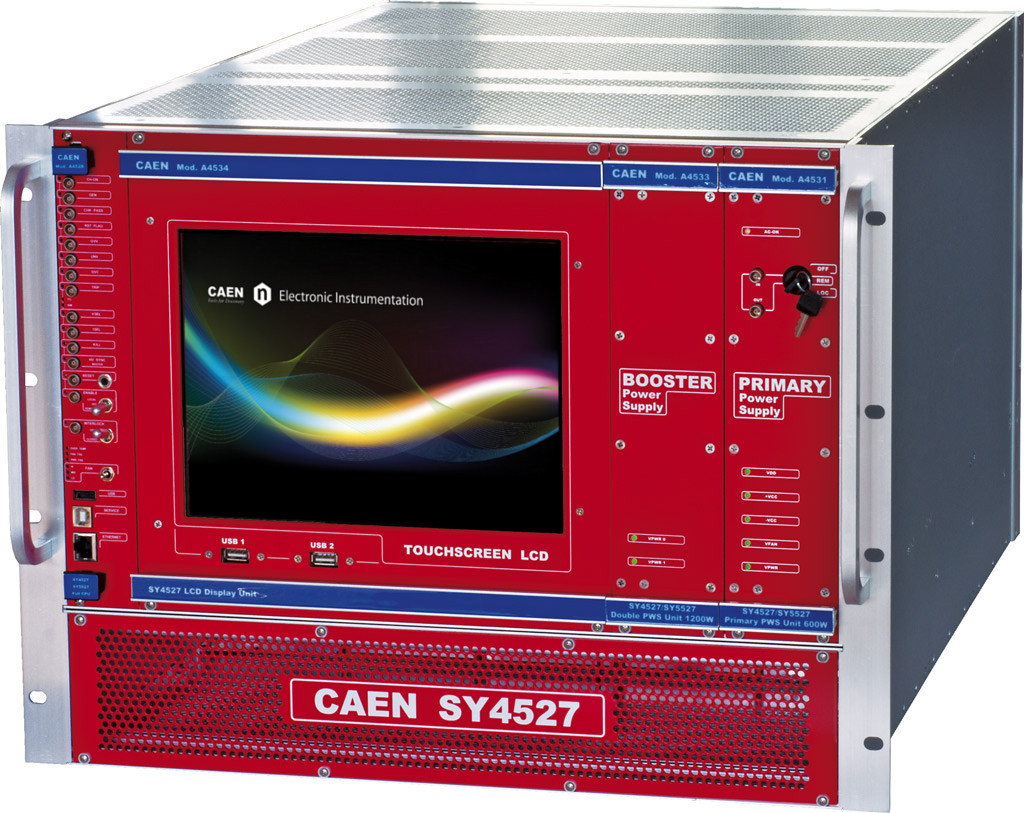
\includegraphics[width=0.55\textwidth]{pics/SY4527n.png}
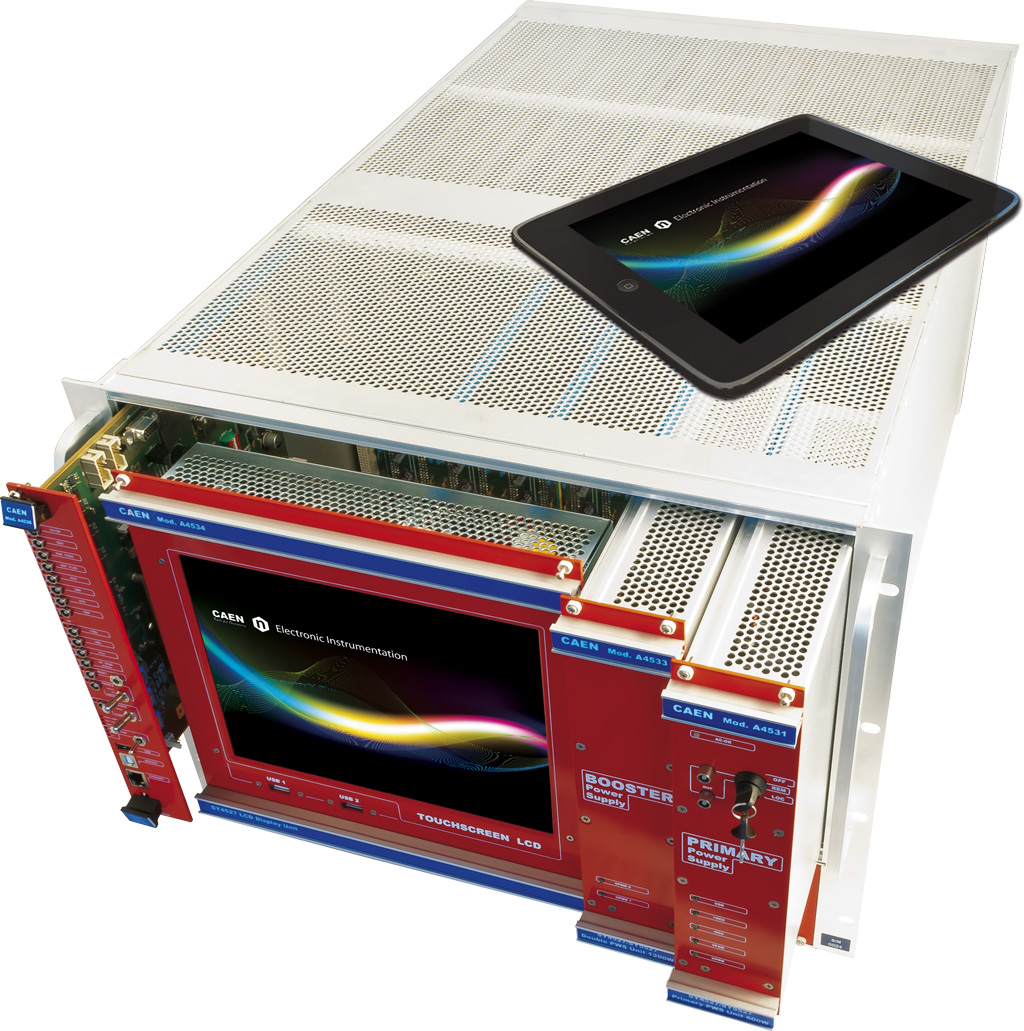
\includegraphics[width=0.55\textwidth]{pics/SY4527_modular.jpg}
\vspace*{0.3cm}
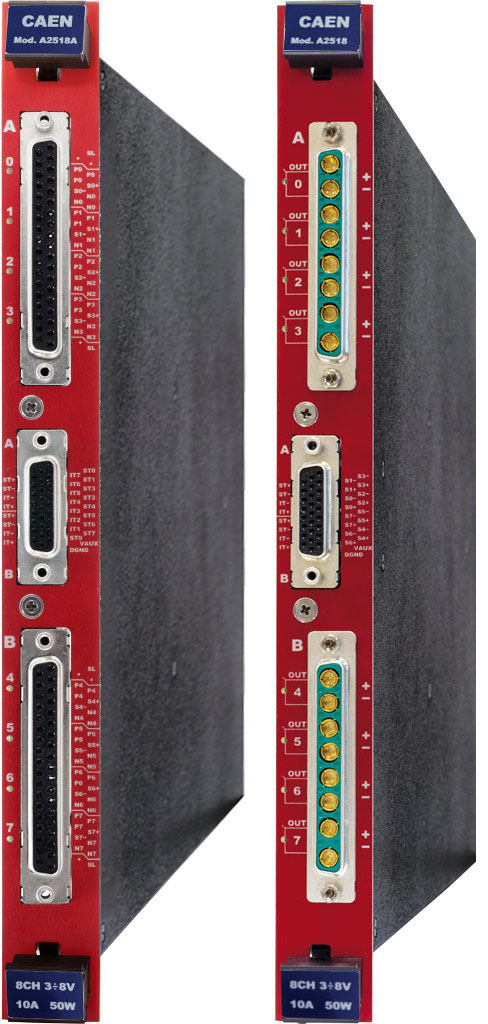
\includegraphics[width=0.21\textwidth]{pics/A2518_1-2.jpg}
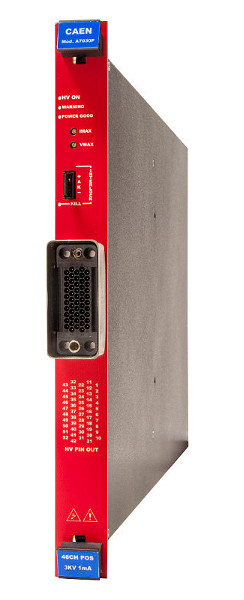
\includegraphics[width=0.18\textwidth]{pics/A7030-panel6.jpg}
\caption{ \label{Fig:SY4527} The CAEN SY4527 power supply.}
\end{figure}

The unit supplies LV and HV power to 138 electronics tiles (RETile), 115 housing 3 MA-PMTs (RETile-3x) 
and 30 housing 2 MA-PMTs (RETile-2x). It runs on EPICS for Slow-Control with same procedures and controls 
already developed for other detectors (i.e. HPS ECAL). It houses:

\vspace*{0.5cm}
\begin{tabular}{llcl} \hline
Nr. & Item & Unit &  Comment \\ \hline
1 & Control board &  A4528    &  With software libraries (EPICS, OPC Server) \\
1 & Power unit    &  A4533    & 1800 watt in total at 220 Volt AC \\
5 & HV Board      &  A1563    & 32 channels, 3kV/1mA, Common Floating Return \\
5 & LV Board      &  A2518    & 8 channels, 8V/10A, Individual Floating \\
5 & Adapter       &  A647     & Radiall (dense) to SHV (robust)  \\\hline
\end{tabular}


\vspace*{0.5cm}
Each HV channel connects one RETile. The HV runs on 138 RG58 cables towards the patch panels mounted 
on the RICH case, and on 138 HTC-50-1-1 cables inside the RICH volume. The HV should be set between 
1000 V (nominal) and 1100 V (maximum). The single channel current dependes on the number of served 
MA-PMTs and should range between 0.5 (RETile-2x) and 0.8 mA (RETile-3x). 

Each LV channel serves four RETiles. The LV runs on 35 AWG16 cables towards the patch panels
connectors (Phoenix 8A) where it is 1:4 splitted into 138 AWG20 copper cables, one per RETile. To 
provide the wanted 5 V at the electronics, the LV should be set in the range between 5.1 and 5.4 V, 
corresponding to the voltage at the patch panel where sense wires provide feedback for
LV stabilization. The LV current per channel should be around 4 A as it supplies about 1 A per 
RETile. The low voltage supply line is designed to not have difficulties to get 
the wanted voltage because of high current. If that is the case contact run coordinator or RICH 
electronic experts.

The low voltage power supply is an Agilent 6621.  It should be set with both channels at $+5$V with their current limits at 6 A, while external wiring inverts one channel to create a bipolar $\pm5$V supply. 
The low voltage supply might have difficulties to get to full voltage because of high current. If that was the case check, with all power supplies off, that all connection are goods. Then contact run coordinator to see if LV power supply addition is possible. 

%%%%%%%%%%%%%%%%%%%%%%%%%%%%%%%%%%%%%%%%%%%%%%%%%%%%%%%%%%%%%%%
%\newpage
{\color{blue}
\section{The RICH Gas Systems}
}

The RICH is serviced by two different gas systems, one for the supply of the nitrogen to be fluxed inside the RICH box and one for the cooling of the FEE.
Both systems are managed through controls and monitors integrated in the CLAS12 software.
The two systems have been dimensioned in such a way that they will be able to serve two RICH modules.


%=============================================================
\subsection{Nitrogen Purge System}

In order to preserve the aerogel optical performance, the RICH box environment must be kept dry by fluxing nitrogen.
The nitrogen system supplies the amount of gas necessary to fill the box (about 5 cubic meters) and to compensate for the gas leakage.
A complete refill of the volume per day is expected under normal operating conditions.
A slight overpressure of 0.5 mbar prevents from the contamination from the outside air.
The system is shown in Fig. \ref{fig:N2_drawing}.
It is based on a 1500 Gallons dewar of liquid nitrogen connected to the RICH box through a on/off valve with a pressure regulator, a 0.01 micron filter to remove all the impurities and flow-meters.
In figure \ref{fig:N2_components}, we report the list of the components of the system.

\vspace*{\stretch{1}}      
\begin{figure}[h!]
\center
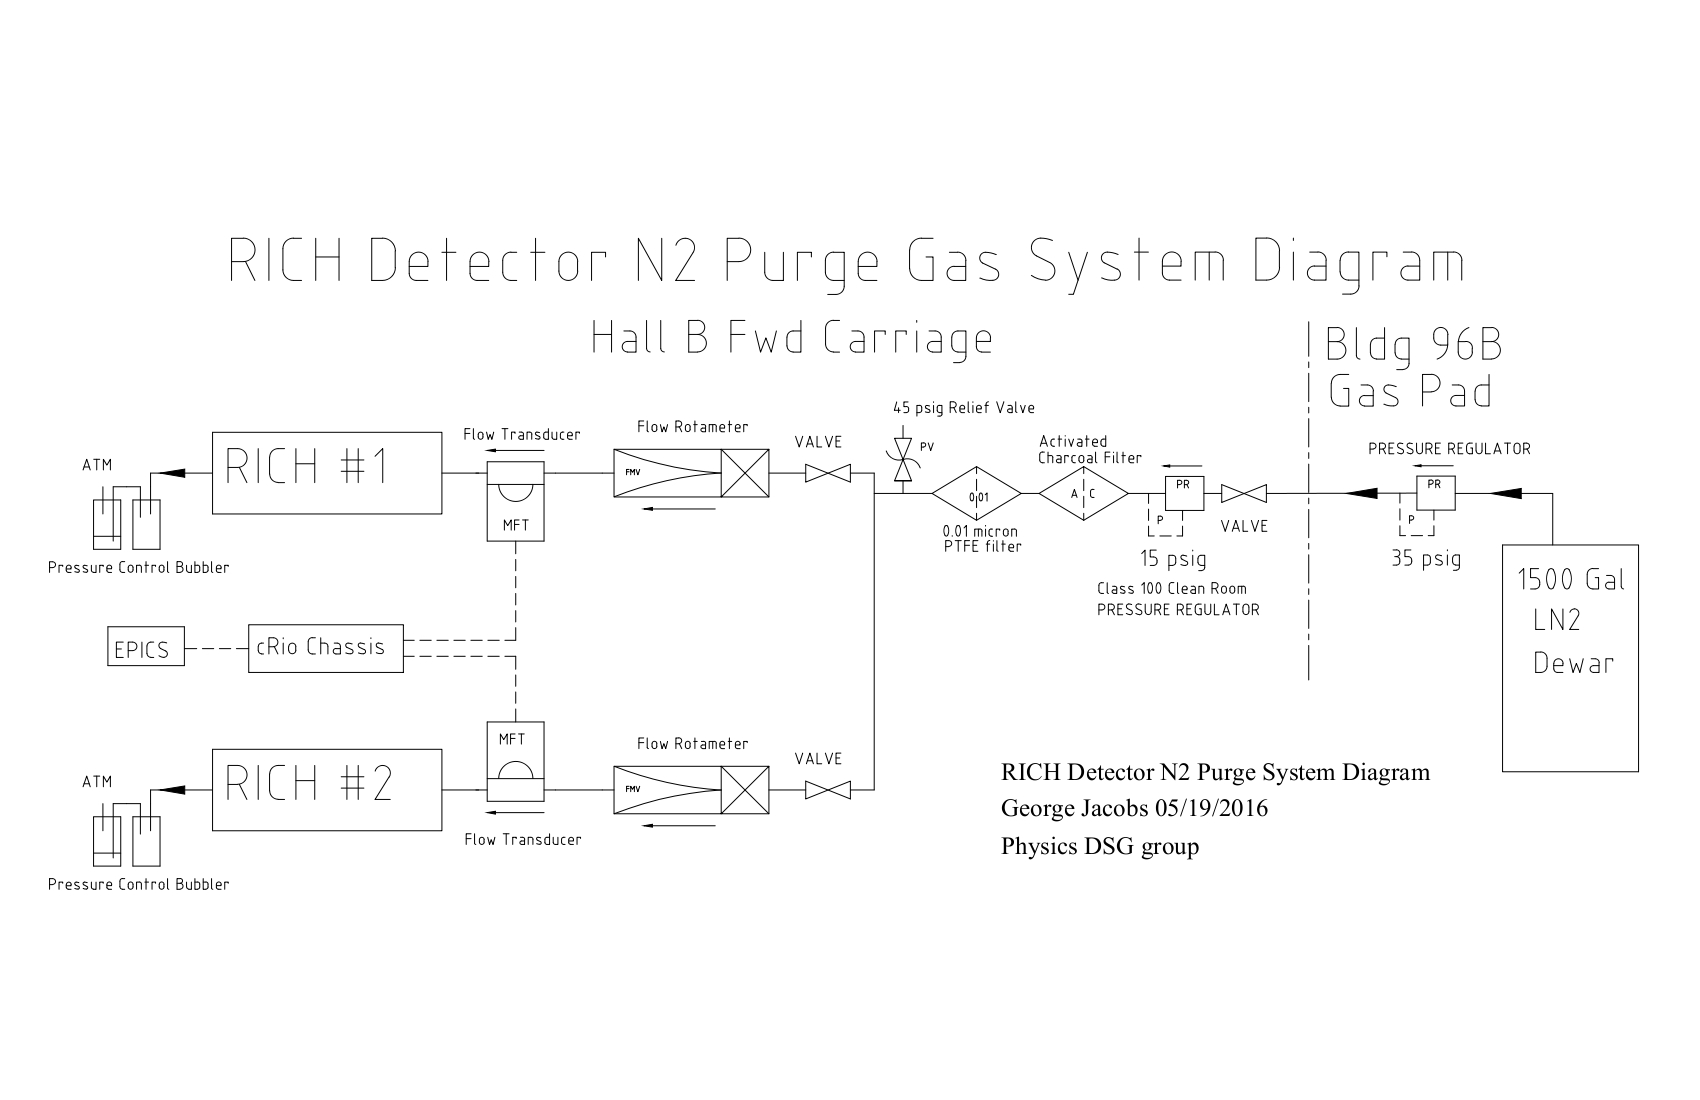
\includegraphics[width=0.99\textwidth]{pics/N2_drawing.jpg}
\caption{ \label{fig:N2_drawing} Schematic of the nitrogen supply system.}
\end{figure}

\vspace*{\stretch{1}}      
\begin{figure}[h!]
\center
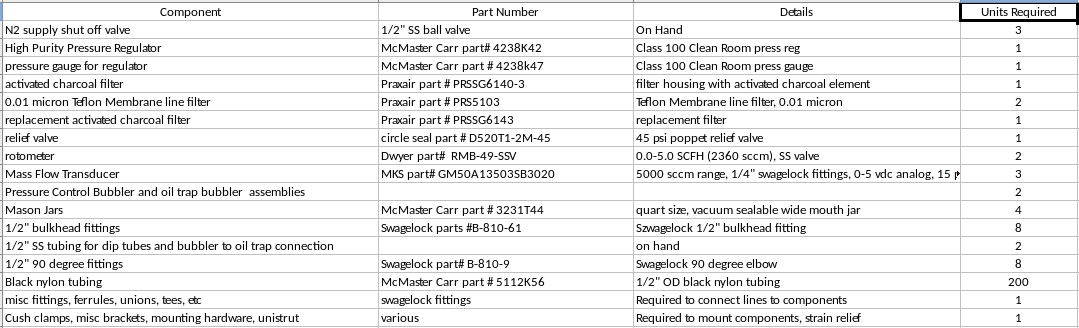
\includegraphics[width=0.99\textwidth]{pics/N2_components.jpg}
\caption{ \label{fig:N2_components} Complete list of the components of the nitrogen supply system.}
\end{figure}



The slow control checks online the correct functionality of the system, i.e.:
\begin{itemize}
\item{Minimum pressure in the liquid nitrogen dewar;}
\item{Minimum flow inside the RICH box;}
\item{Purity of the gas fluxed inside the RICH box.}
\end{itemize}
In the case of failure of the purity control, the valve is automatically turned off and the flow stopped, to prevent possible damage to the aerogel.



%=============================================================
\subsection{The Cooling System}

One tile with two or three MAPMs produces about 3.35 or 3.8 W of heat load, respectively.
The total load in the whole FEE box is 514 W.
This heat load must be dissipated far from the CLAS12 detectors in order to keep the FEE box temperature below 40 $^o$C, the safety limit imposed by the TOF detector which is few cm downstream of the RICH.
%Laboratory have shown that a proper cooling of the system can be obtained by fluxing about 200 liter /min of compressed air.

The FEE RICH cooling system is based on two high capacity air compressors that supply clean dry air at room temperature.
The capacity of each compressor must be large enough so that, in case of failure of one of the two, the other has sufficient capacity to supply the necessary cooling power to two RICH modules.
The compressors charge a 1000 liter capacity air tank.
Air pressure is reduced to supply manual valve flow meters.
In the case of a power outage, the air tank should contain sufficient air to remove the latent heat of the FEE package.
The characteristics of the compressors are shown in table \ref{tab:Compressor}.

\begin{table}[htbp]\centering
    \begin{tabular}{||c|l||}
\hline
\hline
Dimensions & 1.4 x 0.7 x 1.8 m$^3$ \\
\hline
Weight & 515 kg \\
\hline
Max Flow rate  & 1200 l/min \\
\hline
Dew point & 3 $^o$C \\
\hline
Electric power & 10.4 kW \\
\hline
Noise press & 60 dB (A) \\
\hline
\hline
    \end{tabular}
    \caption{The characteristics of the ATLAS Copco SF11-8 MC FF compressors. \label{tab:Compressor}}
\end{table}



Powering up the electronics package inside the RICH without cooling may result in severe damage of the RICH and of other detectors or even fire.
To eliminate this hazard, the RICH HV and LV power supply operations are interlocked to the proper functioning of the cooling system.

A schematic of the RICH cooling system with the interlock circuits is shown in figure \ref{fig:Cooling_interlocks} and the list of its components is reported in figure \ref{fig:Cooling_components}.
It includes a number of temperature sensors installed inside the electronics box, air flow transducers and high purity pressure regulators connected to the inlets and a local pressure regulators on the air tank.
The interlock performs two functions in case of a cooling system failure.
\begin{itemize}
\item{turn off power to the electronic package;}
\item{prevent energizing the electronics package.}
\end{itemize}
There are three cooling cicuit interlocks.
A first interlock requires the minimum of one compressor correctly functioning.
The second interlock requires a minimum air pressure in the tank.
The third interlock require a minimum air flow inside the RICH box.
All three interlocks must be true in order for the electronics package to have power.

\vspace*{\stretch{1}}      
\begin{figure}[h!]
\center
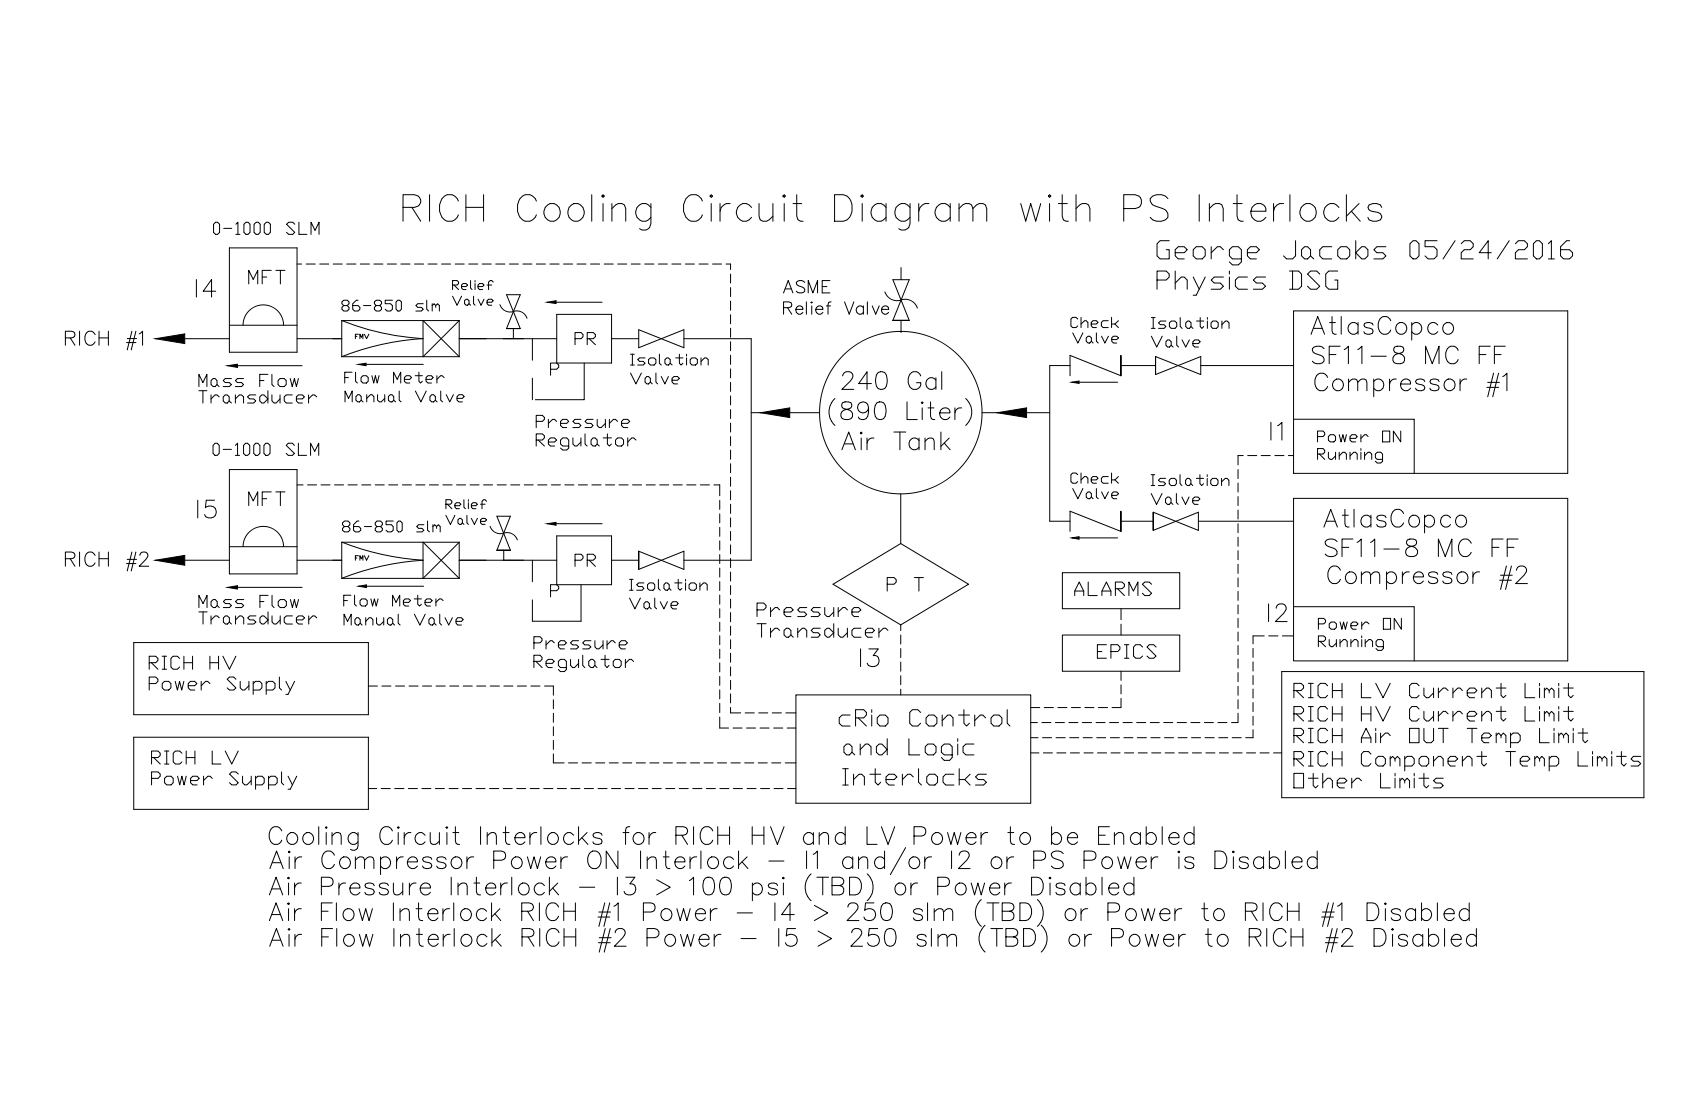
\includegraphics[width=0.99\textwidth]{pics/Cooling_interlocks.jpg}
\caption{ \label{fig:Cooling_interlocks} Schematic of the cooling system and interlocks.}
\end{figure}

\vspace*{\stretch{1}}      
\begin{figure}[h!]
\center
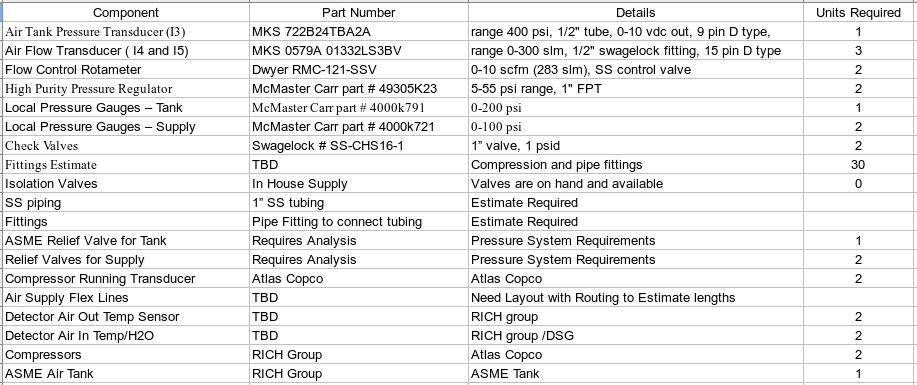
\includegraphics[width=0.99\textwidth]{pics/Cooling_components.jpg}
\caption{ \label{fig:Cooling_components} Complete list of the components of the cooling system and interlocks.}
\end{figure}



%%%%%%%%%%%%%%%%%%%%%%%%%%%%%%%%%%%%%%%%%%%%%%%%%%%%%%%%%%%%%%%
%\newpage
{\color{blue}
\section{The RICH monitors}
}

In this section, we illustrate the general scheme for the RICH operation and monitor controls.
%The RICH slow controls are currently under development.
%Since the RICH uses hardware systems that are also used for other CLAS12 detectors, in some case the GUIs and screenshots showed here are taken from the slow control of detectors that use the same hardware.


%=====================================================
{
 \twocolumn
\subsection{RICH EPICS}
}
\vspace*{\stretch{1}}      
All RICH controls will be  accessible through EPICS, from the main CLAS\_EPICS window (figure~\ref{fig:RICH_EPICSmain}).  If not already running, it can be opened by executing
the command 
\begin{center}
\texttt{clas\_epics}
\end{center}
 in a terminal on any of the \texttt{clonpc\#\#} workstations in the Hall-B counting house.

{\em   All shift workers should be using user \texttt{clasrun} for all instructions in this document.}

The primary RICH screen is shown in figure~\ref{fig:RICH_screen} and opened via the {\bf RICH} button in the right side of the main CLAS EPICS 
screen (figure~\ref{fig:RICH_EPICSmain}).

%From the main CLAS\_EPICS window you can also access individual screens with more controls and details, {\bf Gas system monitoring} in {\it 
%Gas System} then {\it RICH gas System}, the {\bf RICH compressors} in {\it Devices} then {\it RICH Devices}, the {\bf Temperature monitoring} 
%and {\bf Scalers} in {\it RICH Scaler GUI}, the {\bf RICH high voltage} in {\it HV } then {\it RICH HV}.


\vspace*{\stretch{1}}      
\begin{figure}[h!]
\center
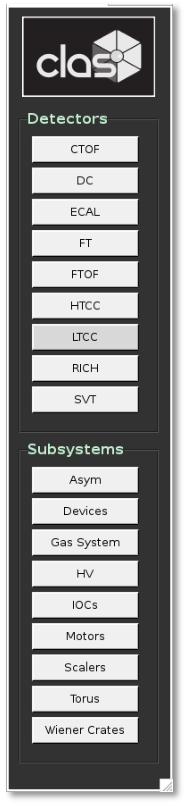
\includegraphics[width=0.28\textwidth]{pics/CLAS_EPICS.pdf}
%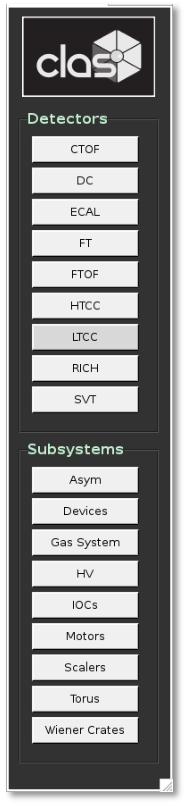
\includegraphics[width=0.38\textwidth]{pics/CLAS_EPICS.pdf}
%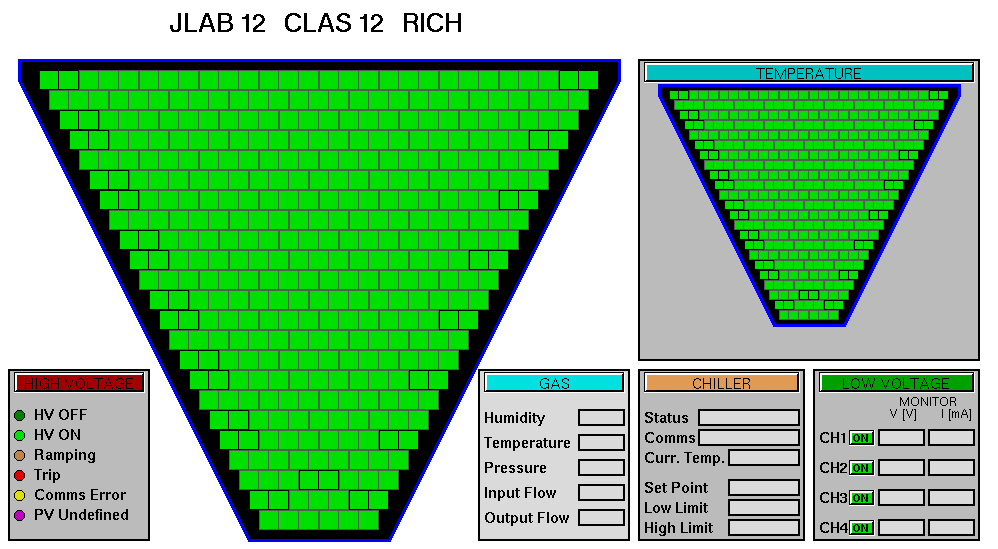
\includegraphics{pics/ElectronicPanel.png}
\caption{ \label{fig:RICH_EPICSmain} View of the Hall-B EPICS main window.}
\end{figure}


\begin{figure}[!htb]
   \begin{minipage}{0.98\textwidth}
     \centering
     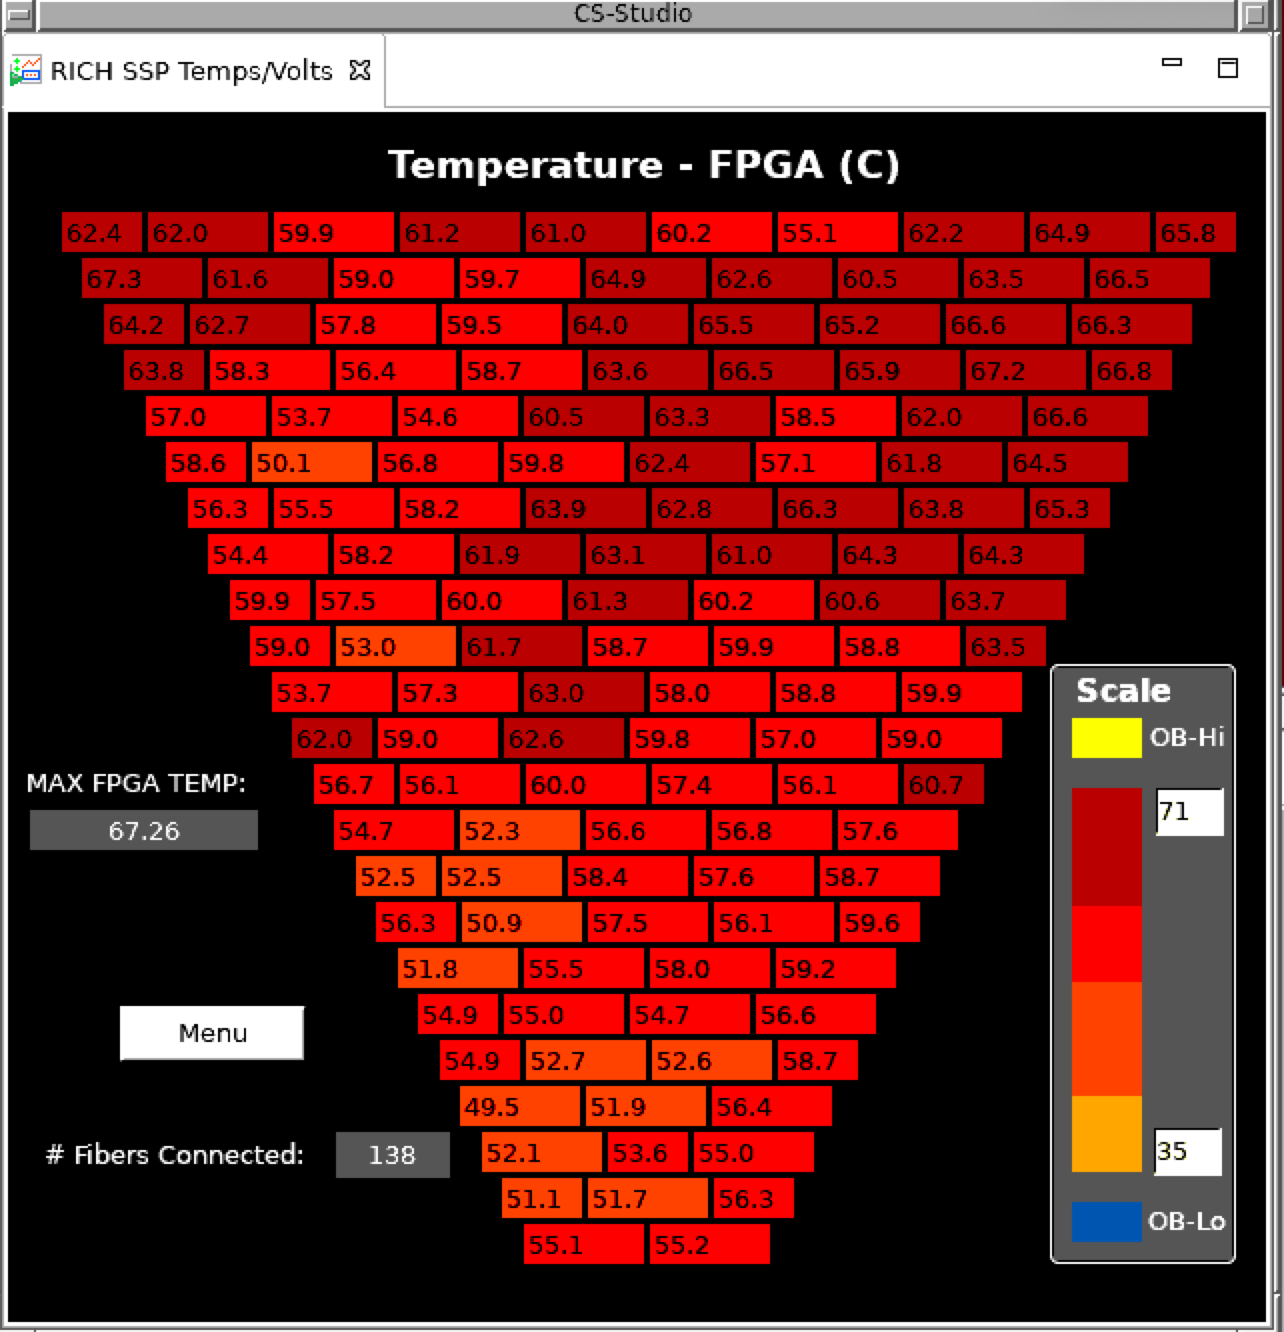
\includegraphics[width=.5\linewidth]{pics/RICH_temp.png}
     \caption{RICH FPGA temperature in $C$.}
     \label{Fig:temp}
   \end{minipage}\hfill
   \begin{minipage}{0.98\textwidth}
     \centering
     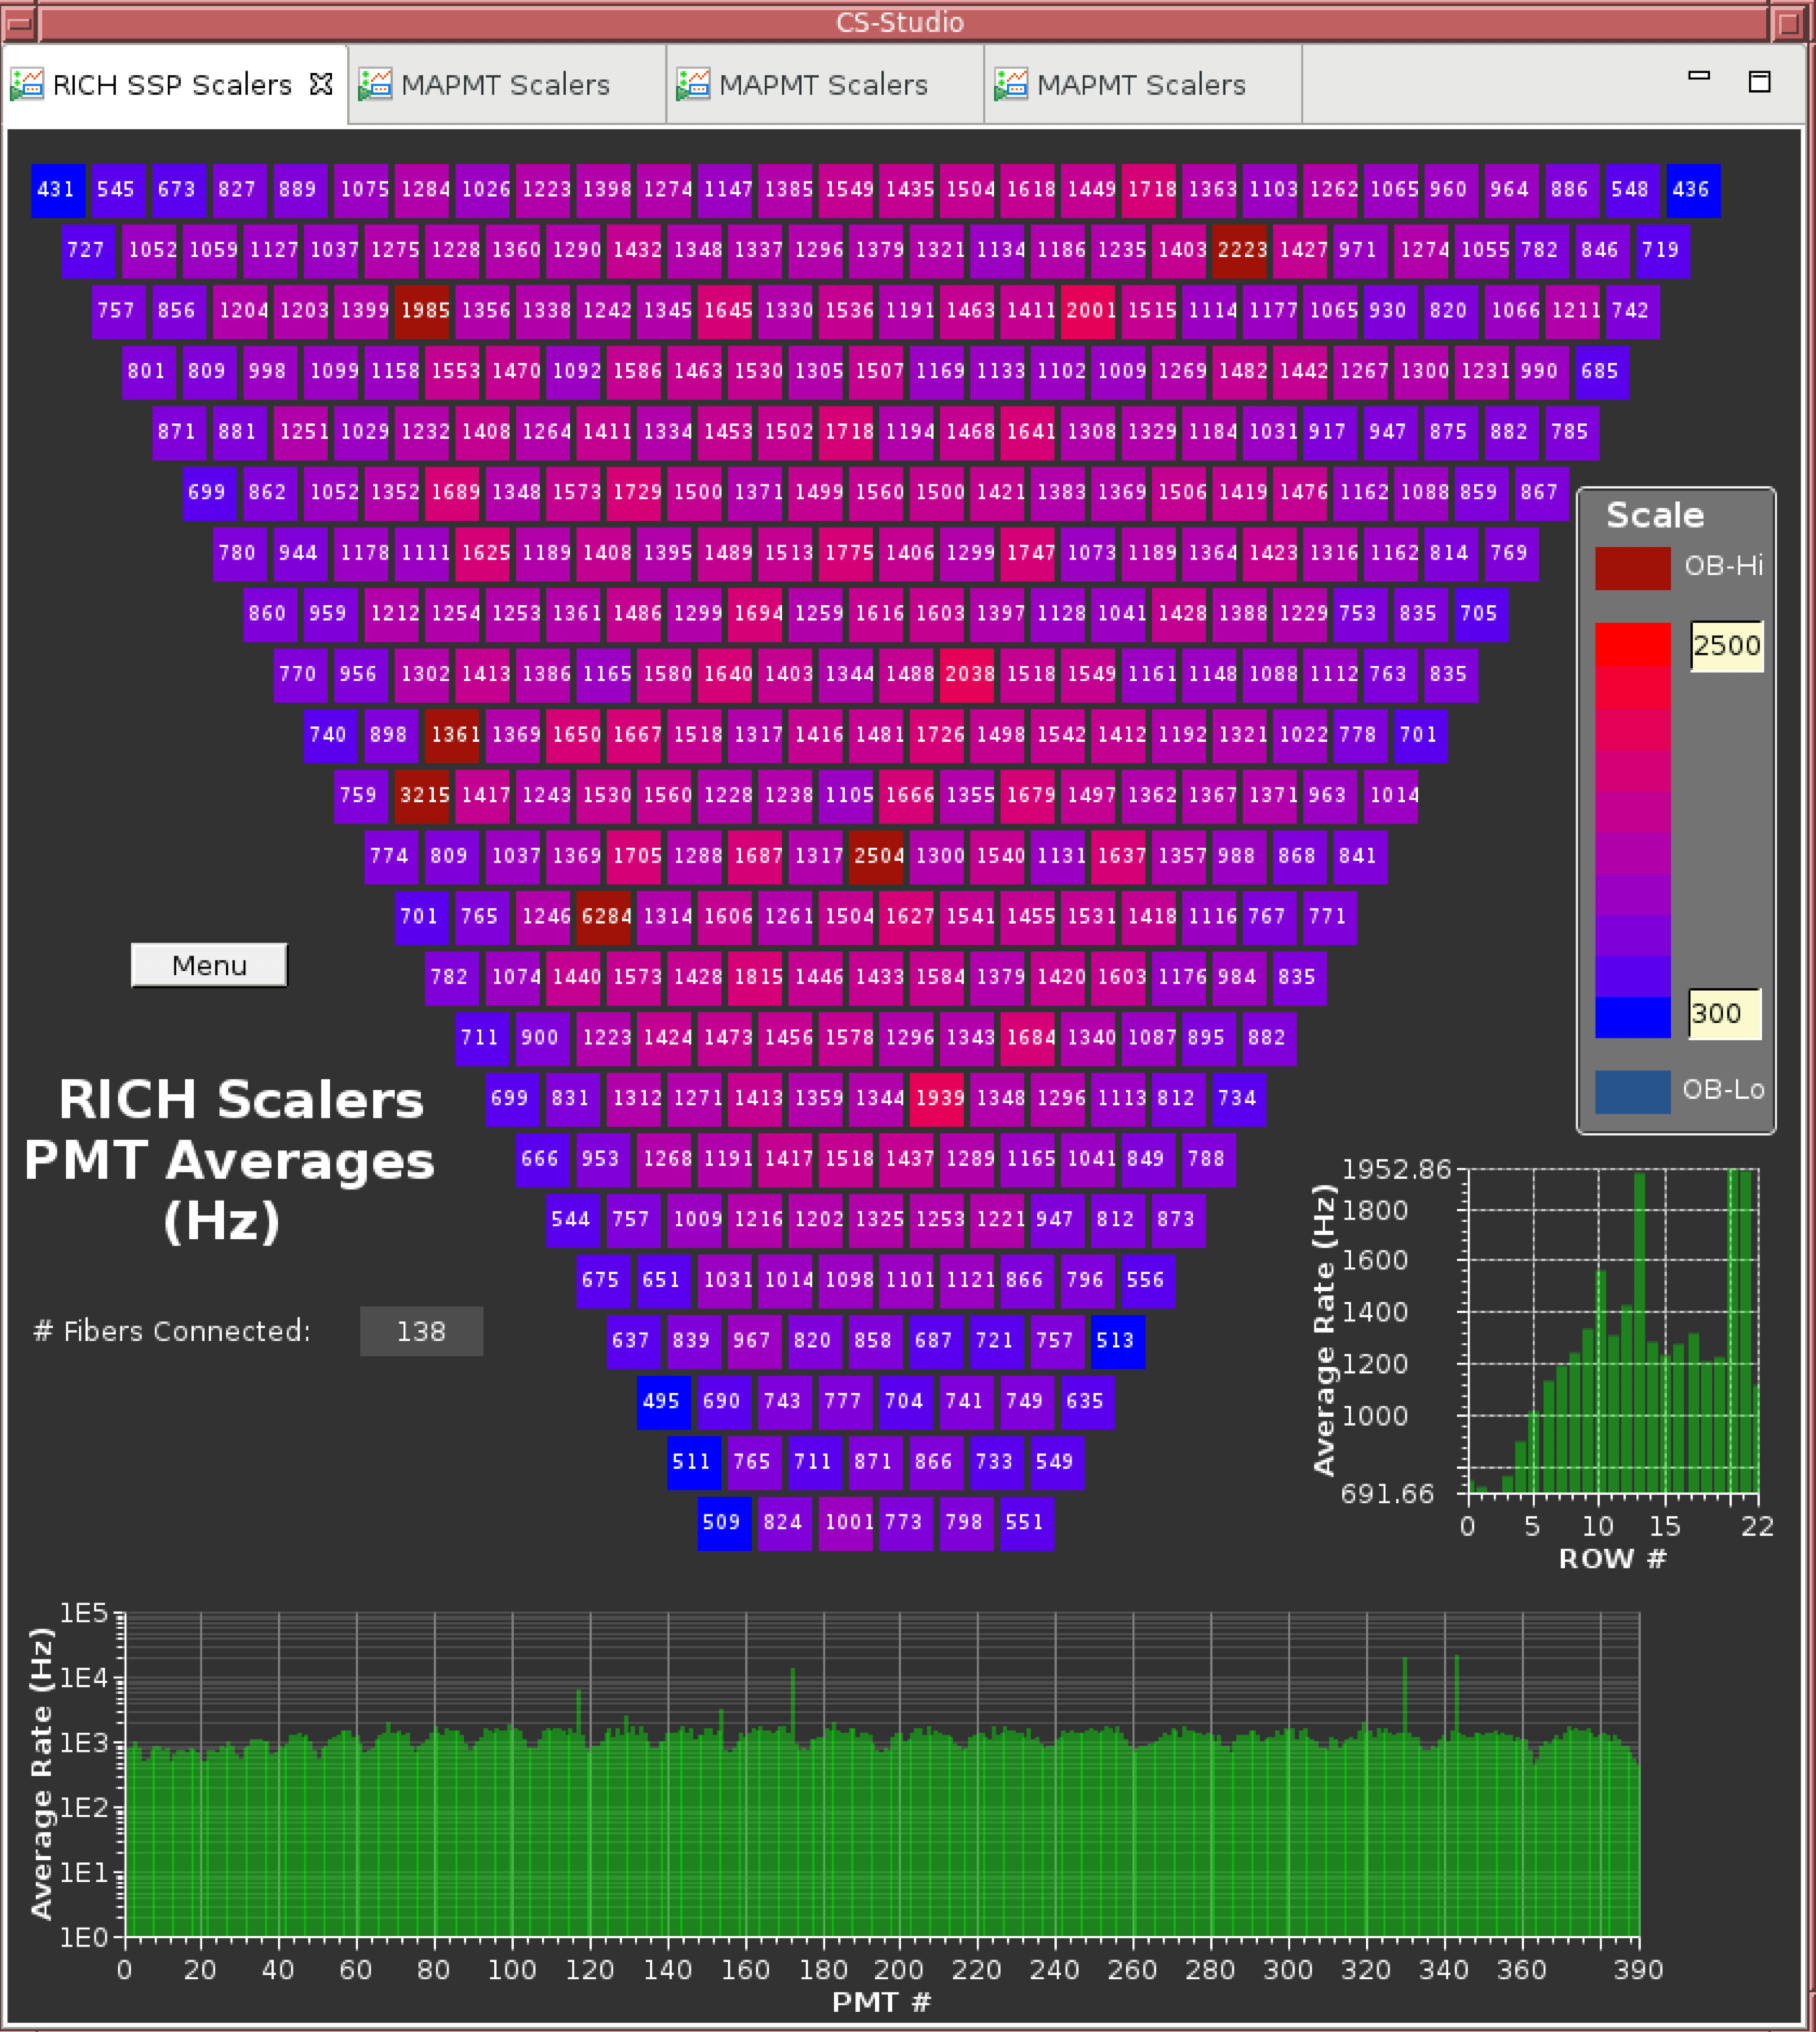
\includegraphics[width=.5\linewidth]{pics/RICH_scalers.png}
     \caption{Average MAPMT's pixels in Hz.}\label{Fig:scaiers}
   \end{minipage}
\end{figure}


 \onecolumn


The main RICH screen combines all basic RICH EPICS controls and monitoring into one window.  It is accessible from the {\bf RICH} 
button in figure~\ref{fig:RICH_EPICSmain}.  This includes embedded versions of the dedicated screens in the following sections:  temperature 
sensors, air-cooling compressors, nitrogen purge system and low and high voltage.  
 
This screen provides the only RICH {\em controls} shift workers should need, which is to turn HV on and off via the red and green 
{\bf ALL ON} and {\bf ALL OFF} buttons.  However, this should be supplemented by the strip charts for temperature and HV current.
%, as well as cctv webcams, for additional {\em monitoring} in the following sections.

%The grey square buttons in the top right of each section of this main RICH screen provide
%access to more detailed or expert screens for the corresponding subsystem.


%begin{figure}[htbp]\centering
%   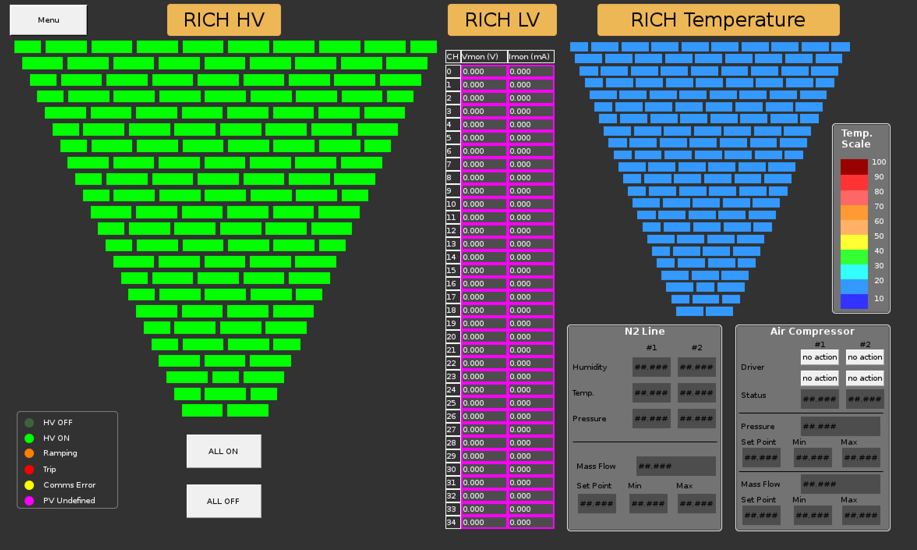
\includegraphics[width=15.5cm]{Justin_plots/MasterScreen.png}
%    \caption{The primary EPICS screen needed for shift workers to monitor RICH.\label{fig:RICH_screen}}
%\end{figure}


%=====================================================
\subsection{Main Slow Control RICH Screens}
The RICH DAQ records the temperature of each of the 138 FPGA chips every few seconds. The normal RICH temperature map
is presented in Figure~\ref{fig:RICH_temp}. 
The average over 64 pixels of the MAPMT rate is presented in Figure~\ref{fig:RICH_scalers}. The maximum temperature is under EPICS control. The RICH alarm will go off in case the temperature will be go over 75C, that is software 


% (and also the main CLAS\_EPICS screen in Figure \ref{fig:RICH_EPICSmain}).
%\begin{figure}[htbp]
%\center
%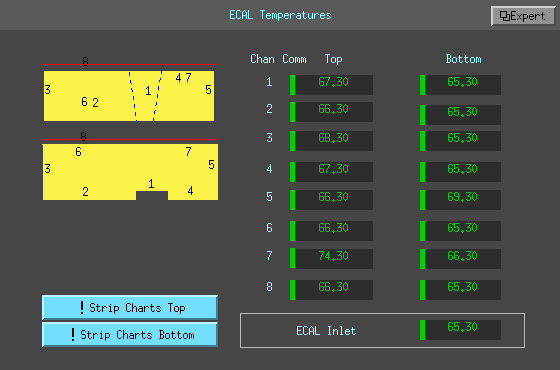
\includegraphics[width=0.5\textwidth]{pics/EcalTemp_2014_12_20.png}
%\caption{ \label{temp} View of the EPICS temperature monitoring window.}
%\end{figure}

%begin{figure}[htbp]
%\center
%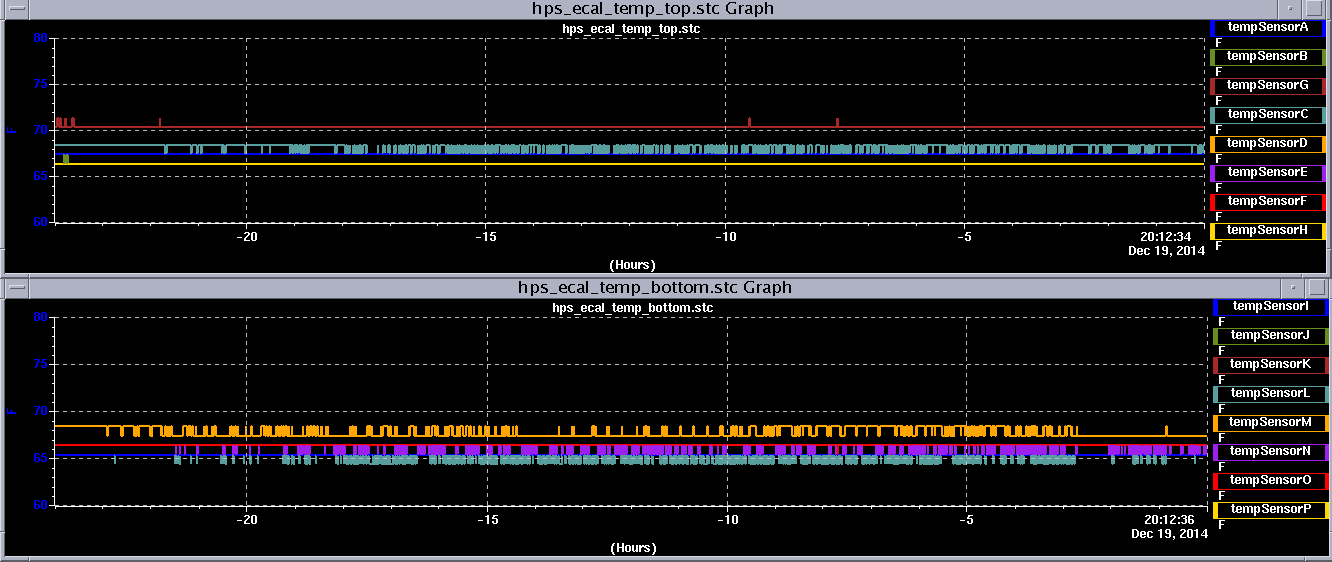
\includegraphics[width=0.45\textwidth,height=4.5cm]{pics/ECal_temp_s.png}
%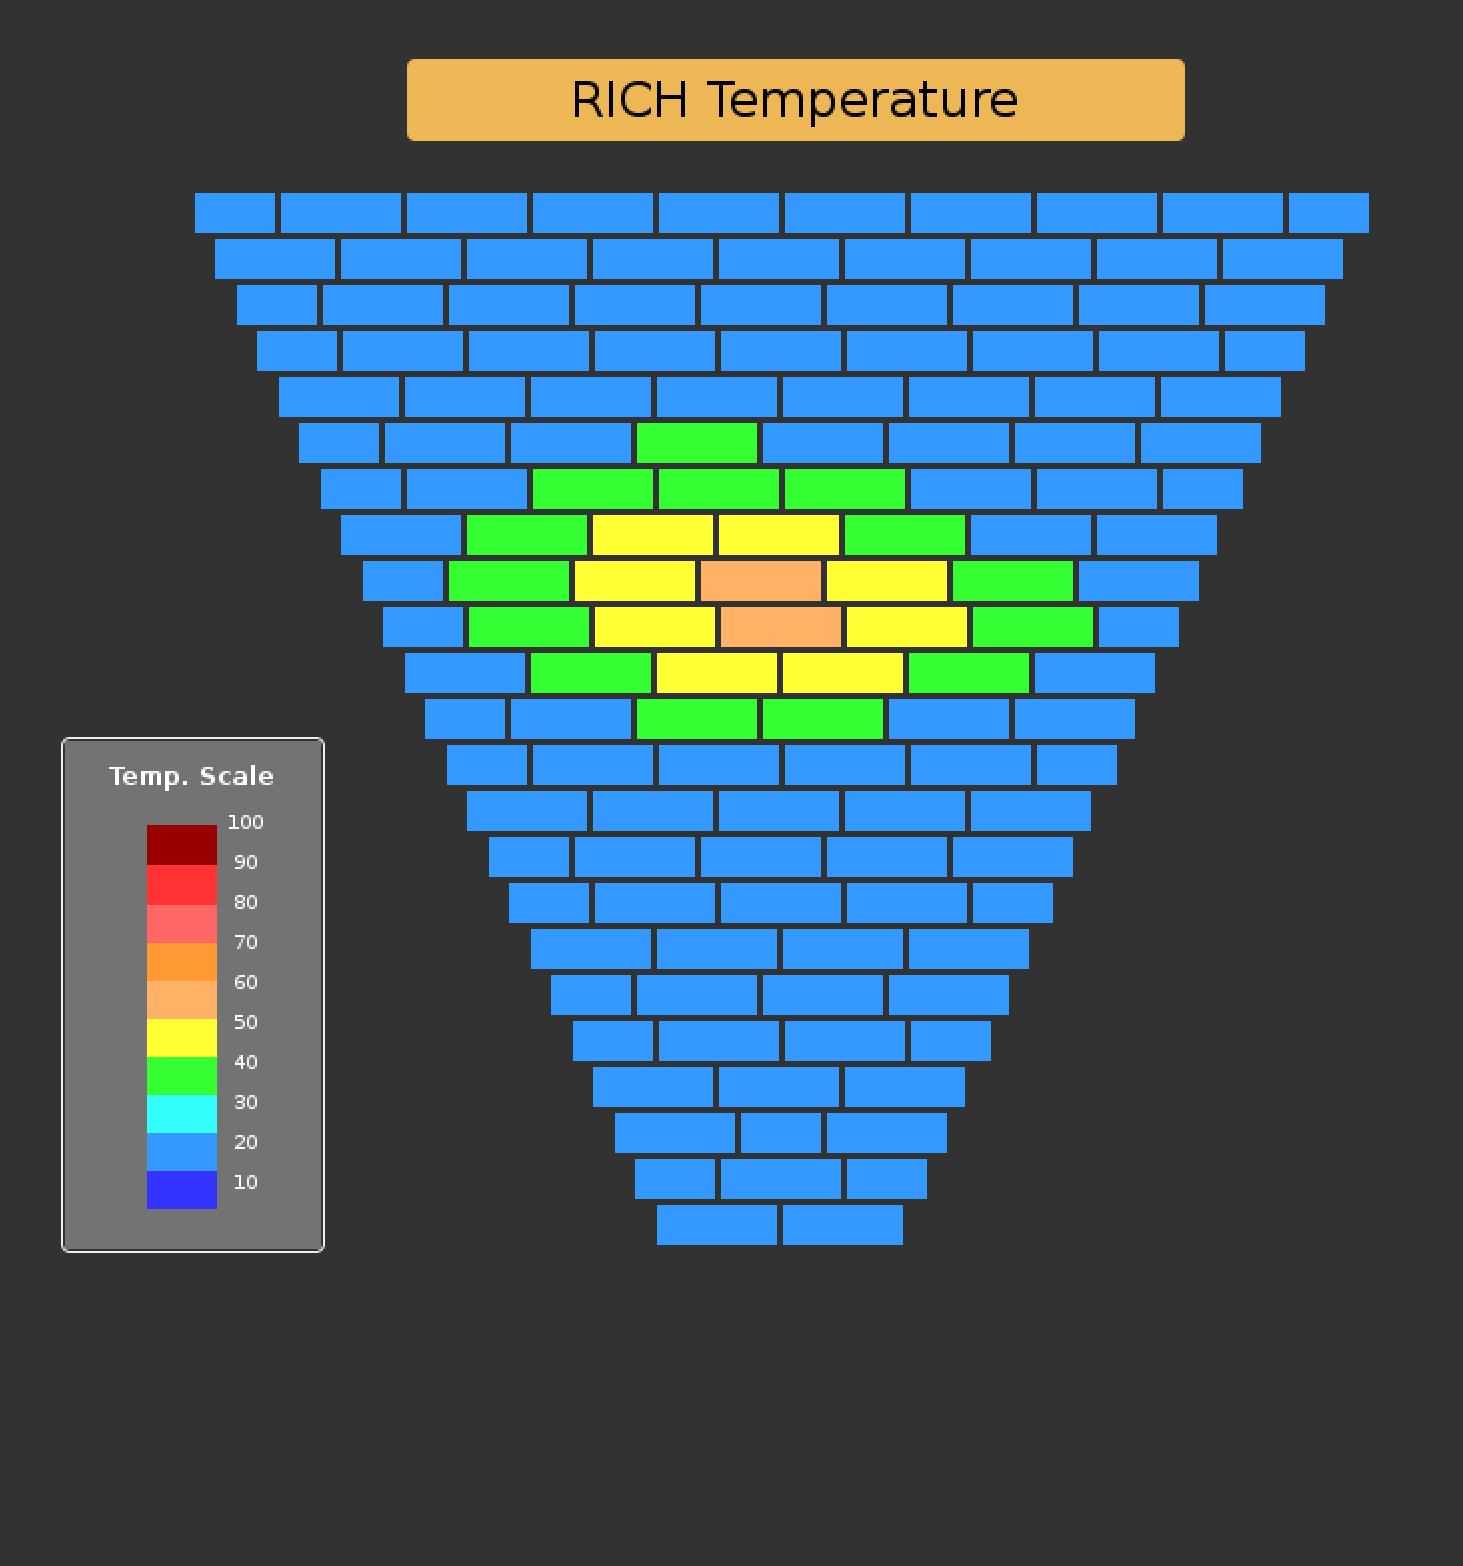
\includegraphics[width=0.3\textwidth,height=4.5cm]{Justin_plots/FireSimulation.PNG}
%\caption{\label{fig:RICH_temperatures} View of the EPICS temperature monitoring strip charts (left) and the temperature portion of the main RICH EPICS screen (right).}
%\end{figure}


%=====================================================
\subsection{Air Cooling System}
The cooling allows to keep the RICH electronic panel at the constant temperature and should be ON at all times. 
In orther to prevent temperature stress on RICH components and adjacent detectors, an interlock prevent the HV and LV power to be active without 
a properly functioning cooling. As other gas systems in Hall-B, the cooling circuit is controlled via a cRio device  and can be monitored through the EPICS controls (figure~\ref{AIR_gas}).
Shift takers should not attempt to change the cooling system settings and call RICH expert 
in case of problem.  %The webcam is accessible in a web browser via the url \texttt{cctv10.jlab.org} and the ``Monitoring'' tab on the {\bf CLAS Run Wiki}.

\begin{figure}[htbp]
\center
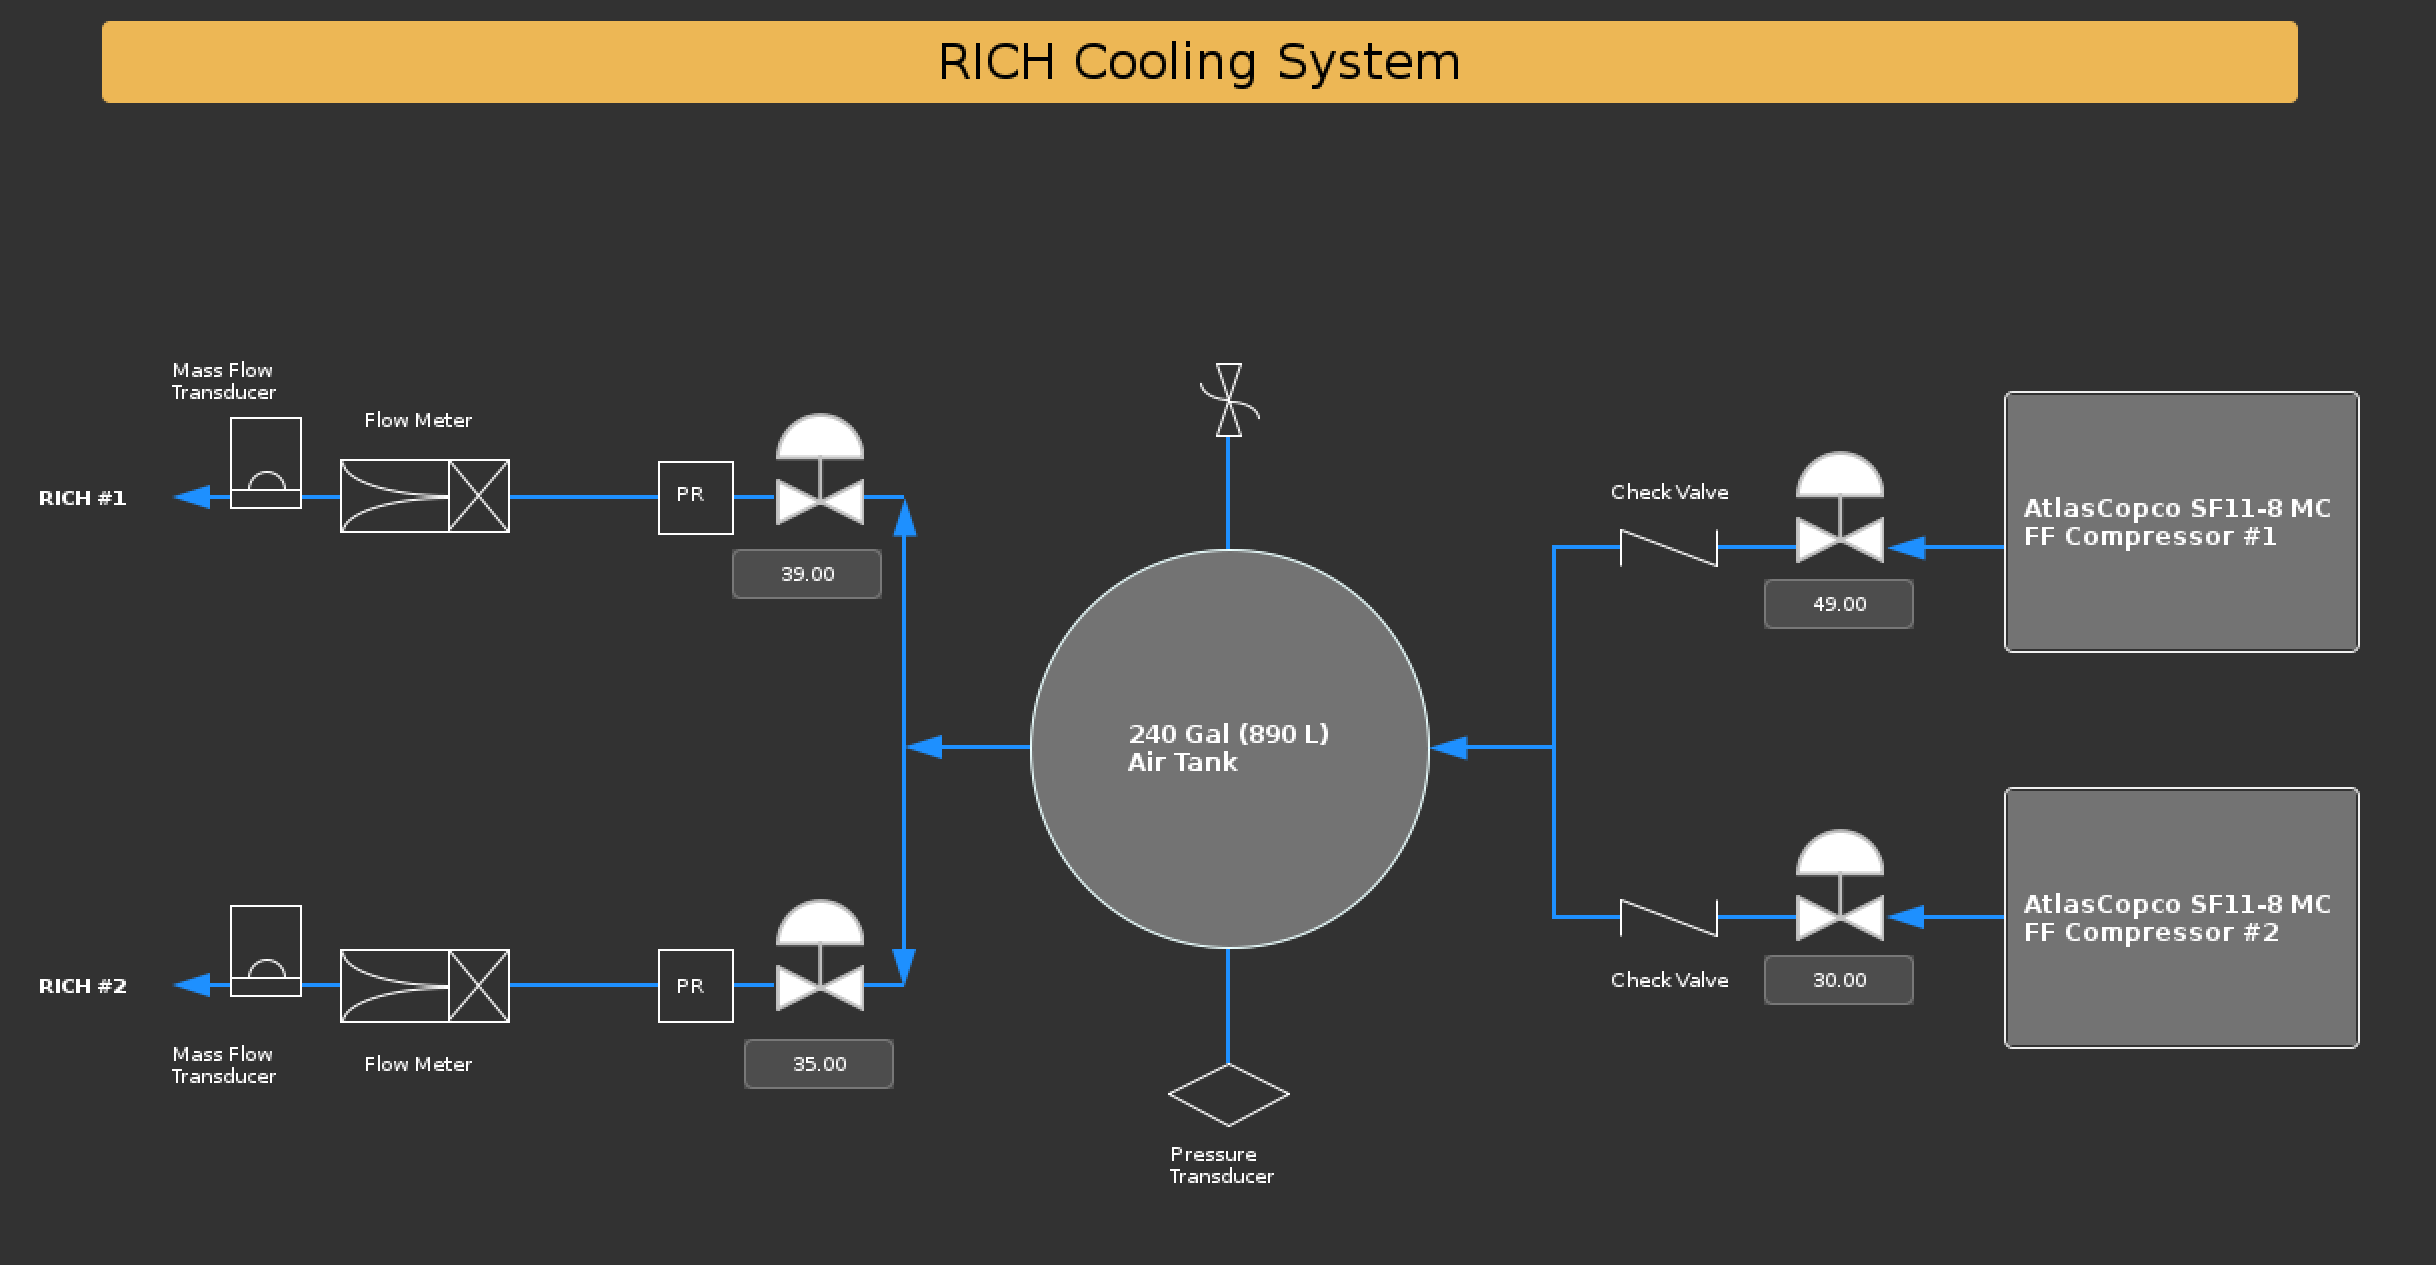
\includegraphics[width=0.80\textwidth]{Justin_plots/GasCooling.PNG}
\caption{ \label{AIR_gas} RICH air cooling system control.}
\end{figure}

%\begin{figure}[htbp]
%\center
%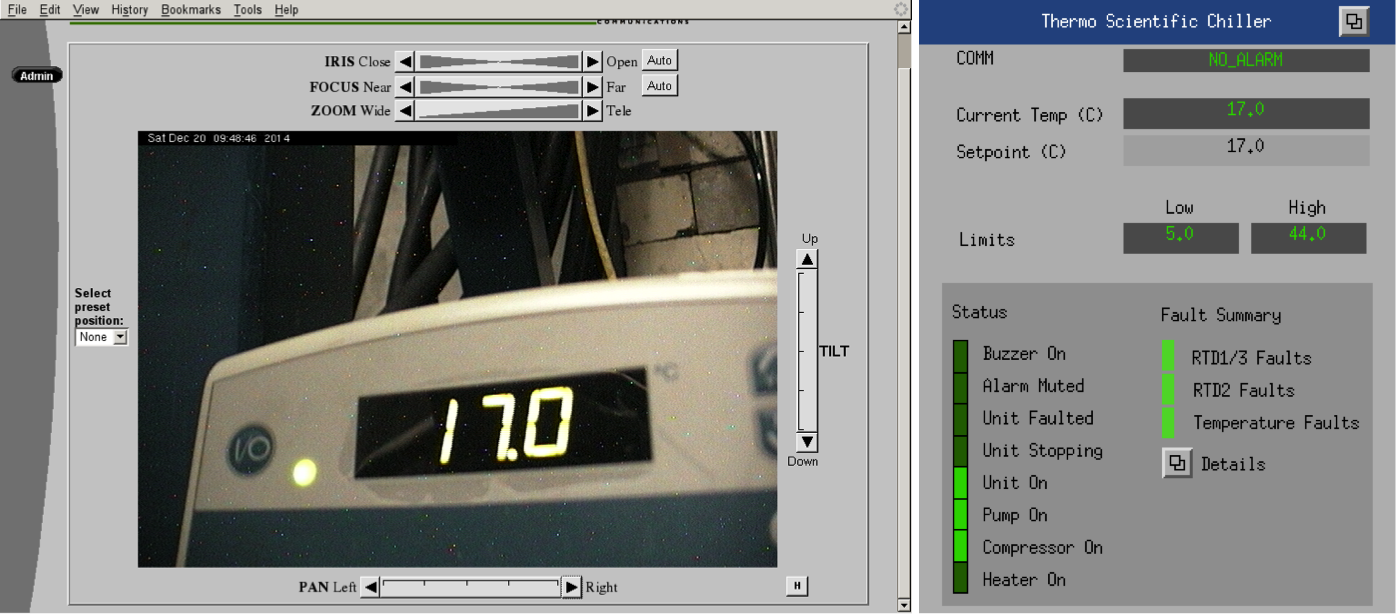
\includegraphics[width=0.99\textwidth]{pics/ChillerCombo.png}
%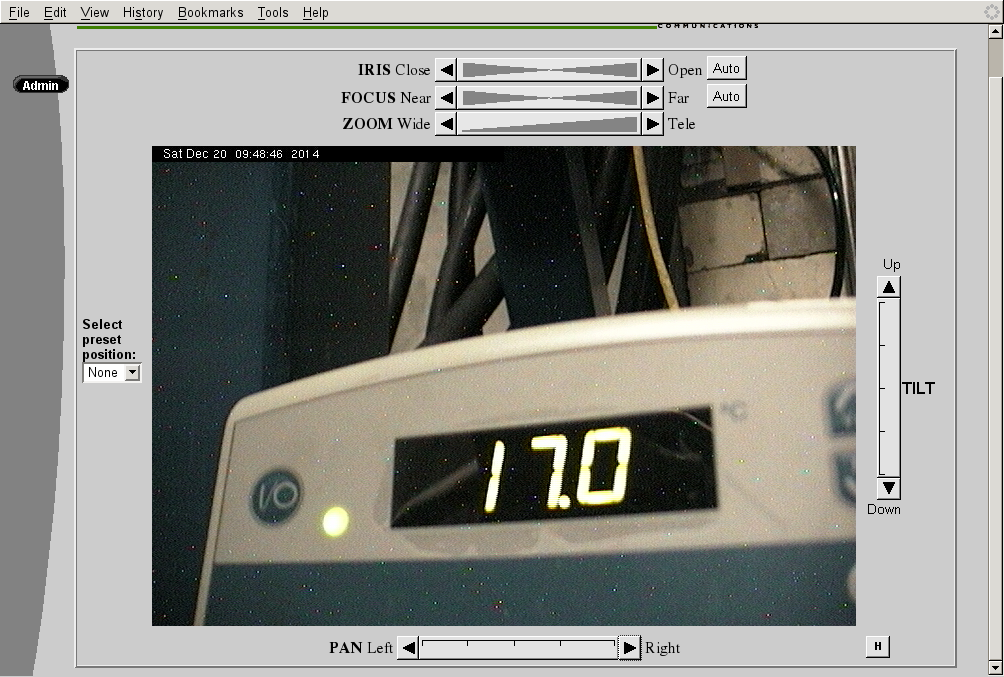
\includegraphics[width=0.45\textwidth,height=4.5cm]{pics/ChillerCam_2014_12_20.png}
%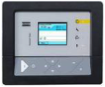
\includegraphics[width=0.45\textwidth,height=4.5cm]{pics/RICH_chillerdisplay.png}
%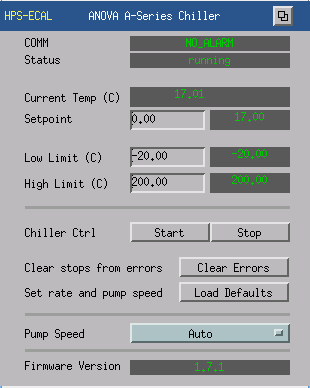
\includegraphics[width=0.3\textwidth,height=5.5cm]{pics/ChillerWin_2016_1_17.png}
%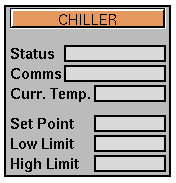
\includegraphics[width=0.3\textwidth,height=4.5cm]{pics/epics_rich_chiller.png}
%\caption{ \label{ChillerCam} View of the air-cooling compressor display (left) and its portion of the main RICH EPICS window (right).}
%\end{figure}

\subsection{Nitrogen Purge System}

In order to preserve the aerogel optical performance, the RICH box environment must be kept dry by fluxing nitrogen.
The EPICS control screen is shown on Fig. \ref{fig:N2_drawing}.


\vspace*{\stretch{1}}      
\begin{figure}[h!]
\center
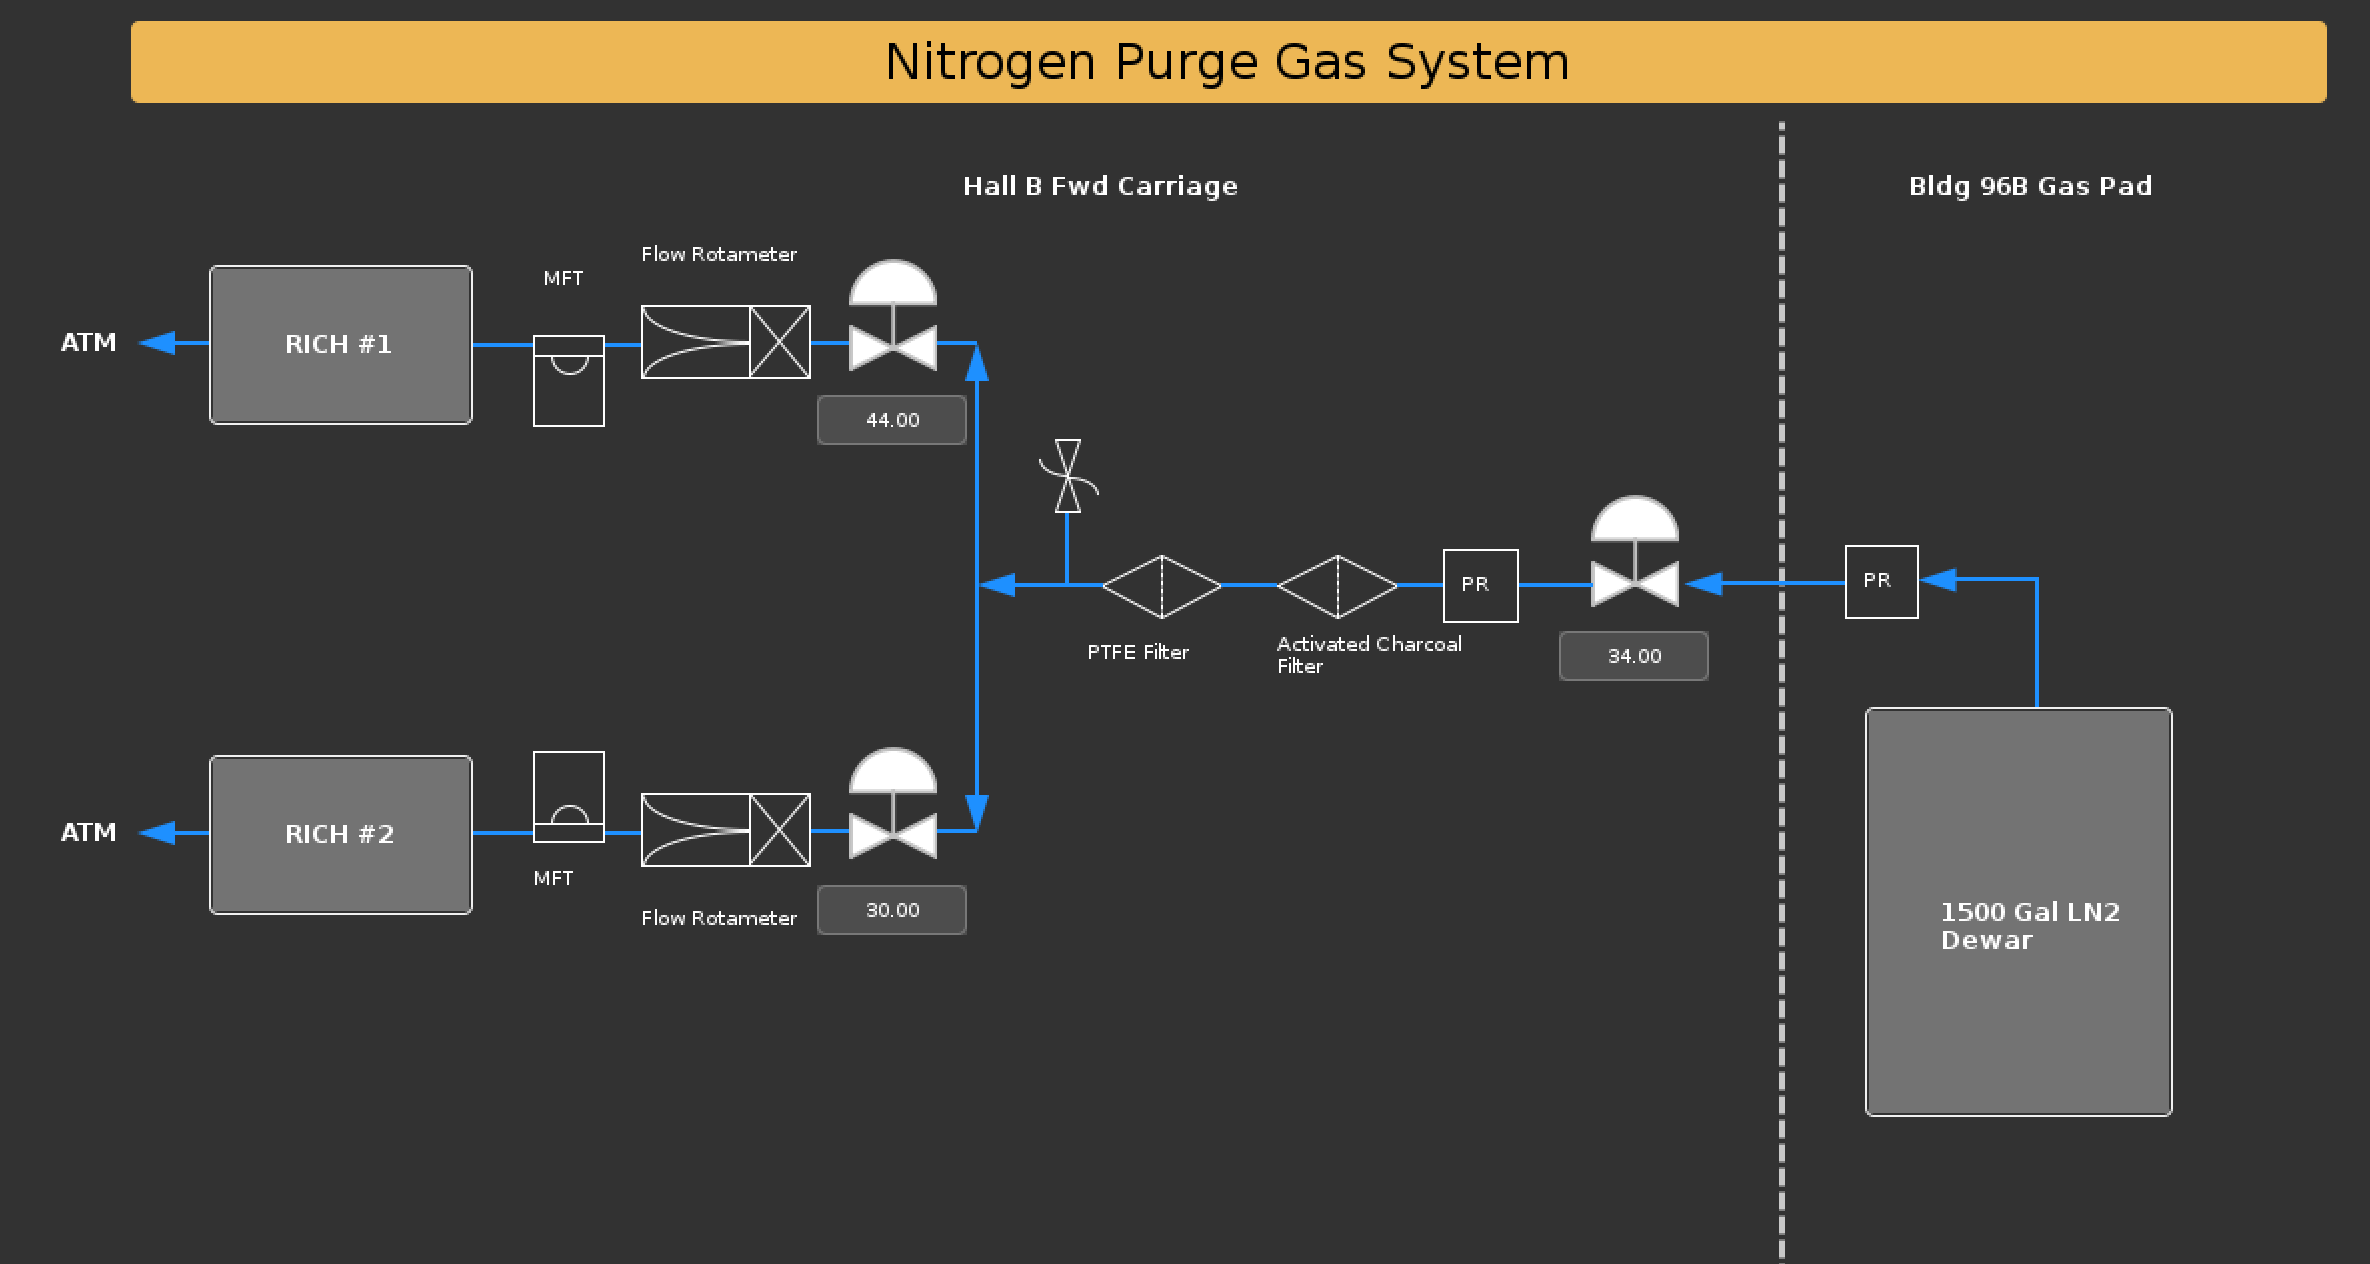
\includegraphics[width=0.99\textwidth]{Justin_plots/N2Purge.PNG}
\caption{ \label{fig:N2_drawing} RICH  nitrogen supply system control.}
\end{figure}

%=====================================================
\subsection{ Low Voltage Control}

The low voltage supply of the RICH is controlled and monitored using the main RICH
EPICS window (Figure ~\ref{fig:RICH_screen}). It has buttons to ramp up and down the entire 
RICH voltages (labeled {\bf ALL ON} and {\bf ALL OFF}), open windows for
individual channel control (see  figure~\ref{LVControl}), and open more detailed expert views.

\begin{figure}[htbp]
\center
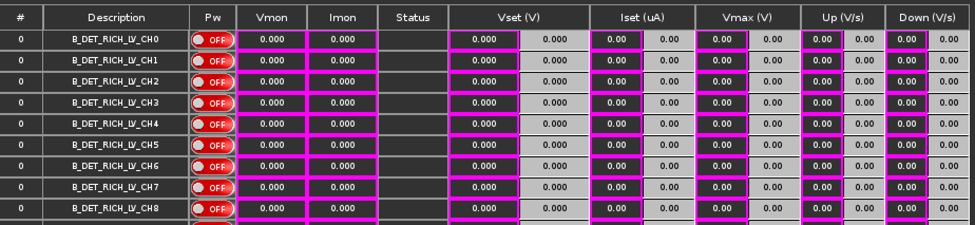
\includegraphics[width=0.99\textwidth]{Justin_plots/LVallChannels.png}
\caption{ \label{LVControl} Cropped view of the EPICS LV control window for individual channels of the RICH detector.}
\end{figure}

%=====================================================
\subsection{ High Voltage Control}

The high voltage supply of the RICH is controlled and monitored using the main RICH
EPICS window (Figure ~\ref{fig:RICH_screen}).  It has buttons to ramp up and down the entire 
RICH voltages (labeled {\bf ALL ON} and {\bf ALL OFF}), open windows for
individual channel control, and open more detailed expert views (see Fig. \ref{HVControl}).
\begin{figure}[htbp]
\center
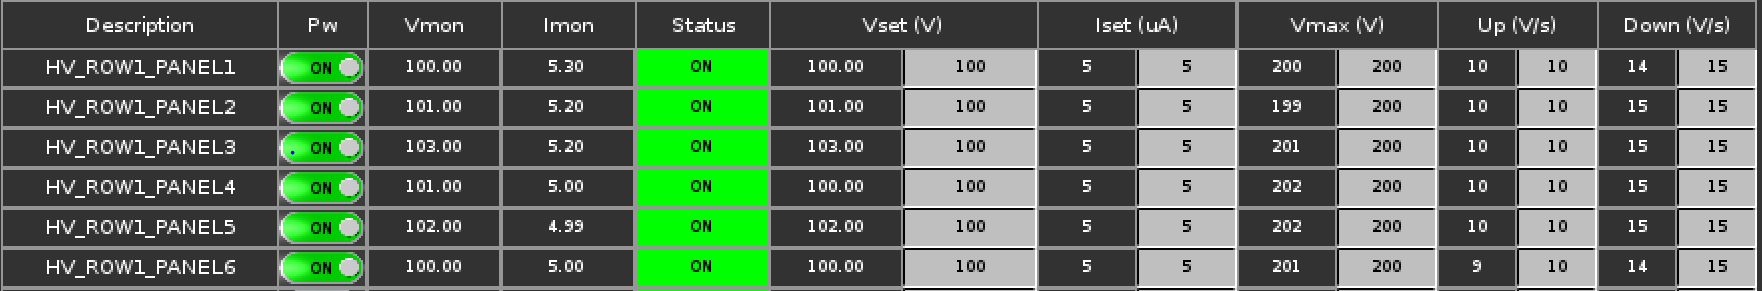
\includegraphics[width=0.99\textwidth]{Justin_plots/HVControlsNumbers.PNG}
\caption{ \label{HVControl} Cropped view of the EPICS HV control window for individual channels of the RICH detector.}
\end{figure}

%(e.g. figure ~\ref{HV}).

%%%%%%%%%%%%%%%%%%%%%%%%%%%%%%%%%%%%%%%%%%%%%%%%%%%%
%{\color{blue}
%\section{The RICH operation}
%}


%%%%%%%%%%%%%%%%%%%%%%%%%%%%%%%%%%%%%%%%%%%%%%%%%%%%%%%%%%%%%%%%%%%%%%%%%%%%%
%%%%%%%%%%%%%%%%%%%%%%%%%%%%%%%%%%%%%%%%%%%%%%%%%%%%%%%%%%%%%%%%%%%%%%%%%%%%%
%%%%%%%%%%%%%%%%%%%%%%%%%%%%%%%%%%%%%%%%%%%%%%%%%%%%%%%%%%%%%%%%%%%%%%%%%%%%%
%%%%%%%%%%%%%%%%%%%%%%%%%%%%%%%%%%%%%%%%%%%%%%%%%%%%%%%%%%%%%%%%%%%%%%%%%%%%%
%%%%%%%%%%%%%%%%%%%%%%%%%%%%%%%%%%%%%%%%%%%%%%%%%%%%%%%%%%%%%%%%%%%%%%%%%%%%%
%%%%%%%%%%%%%%%%%%%%%%%%%%%%%%%%%%%%%%%%%%%%%%%%%%%%%%%%%%%%%%%%%%%%%%%%%%%%%

\end{document}
 ib pics/